\documentclass[a4paper,14pt,oneside,openany]{memoir}

%%% Задаем поля, отступы и межстрочный интервал %%%

\usepackage[left=30mm, right=15mm, top=20mm, bottom=20mm]{geometry} % Пакет geometry с аргументами для определения полей
\pagestyle{plain} % Убираем стандарные для данного класса верхние колонтитулы с заголовком текущей главы, оставляем только номер страницы снизу по центру
\parindent=1.25cm % Абзацный отступ 1.25 см, приблизительно равно пяти знакам, как по ГОСТ
\usepackage{indentfirst} % Добавляем отступ к первому абзацу
%\linespread{1.3} % Межстрочный интервал (наиболее близко к вордовскому полуторному) - тут вместо этого используется команда OnehalfSpacing*

%%% Задаем языковые параметры и шрифт %%%

\usepackage[english, russian]{babel}                % Настройки для русского языка как основного в тексте
% \babelfont{rm}{Times New Roman}                     % TMR в качестве базового roman-щрифта

%%% Задаем стиль заголовков и подзаголовков в тексте %%%

\setsecnumdepth{subsection} % Номера разделов считать до третьего уровня включительно, т.е. нумеруются только главы, секции, подсекции
\renewcommand*{\chapterheadstart}{} % Переопределяем команду, задающую отступ над заголовком, чтобы отступа не было
\renewcommand*{\printchaptername}{} % Переопределяем команду, печатающую слово "Глава", чтобы оно не печалось
%\renewcommand*{\printchapternum}{} % То же самое для номера главы - тут не надо, номер главы оставляем
\renewcommand*{\chapnumfont}{\normalfont\bfseries} % Меняем стиль шрифта для номера главы: нормальный размер, полужирный
\renewcommand*{\afterchapternum}{\hspace{1em}} % Меняем разделитель между номером главы и названием
\renewcommand*{\printchaptertitle}{\normalfont\bfseries\centering\MakeUppercase} % Меняем стиль написания для заголовка главы: нормальный размер, полужирный, центрированный, заглавными буквами
\setbeforesecskip{20pt} % Задаем отступ перед заголовком секции
\setaftersecskip{20pt} % Ставим такой же отступ после заголовка секции
\setsecheadstyle{\raggedright\normalfont\bfseries} % Меняем стиль написания для заголовка секции: выравнивание по правому краю без переносов, нормальный размер, полужирный
\setbeforesubsecskip{20pt} % Задаем отступ перед заголовком подсекции
\setaftersubsecskip{20pt} % Ставим такой же отступ после заголовка подсекции
\setsubsecheadstyle{\raggedright\normalfont\bfseries}  % Меняем стиль написания для заголовка подсекции: выравнивание по правому краю без переносов, нормальный размер, полужирный

%%% Задаем параметры оглавления %%%

\addto\captionsrussian{\renewcommand\contentsname{Содержание}} % Меняем слово "Оглавление" на "Содержание"
\setrmarg{2.55em plus1fil} % Запрещаем переносы слов в оглавлении
%\setlength{\cftbeforechapterskip}{0pt} % Эта команда убирает интервал между заголовками глав - тут не надо, так красивее смотрится
\renewcommand{\aftertoctitle}{\afterchaptertitle \vspace{-\cftbeforechapterskip}} % Делаем отступ между словом "Содержание" и первой строкой таким же, как у заголовков глав
%\renewcommand*{\chapternumberline}[1]{} % Делаем так, чтобы номер главы не печатался - тут не надо
\renewcommand*{\cftchapternumwidth}{1.5em} % Ставим подходящий по размеру разделитель между номером главы и самим заголовком
\renewcommand*{\cftchapterfont}{\normalfont\MakeUppercase} % Названия глав обычным шрифтом заглавными буквами
\renewcommand*{\cftchapterpagefont}{\normalfont} % Номера страниц обычным шрифтом
\renewcommand*{\cftchapterdotsep}{\cftdotsep} % Делаем точки до номера страницы после названий глав
\renewcommand*{\cftdotsep}{1} % Задаем расстояние между точками
\renewcommand*{\cftchapterleader}{\cftdotfill{\cftchapterdotsep}} % Делаем точки стандартной формы (по умолчанию они "жирные")
\maxtocdepth{subsection} % В оглавление попадают только разделы первыхтрех уровней: главы, секции и подсекции

%%% Выравнивание и переносы %%%

%% http://tex.stackexchange.com/questions/241343/what-is-the-meaning-of-fussy-sloppy-emergencystretch-tolerance-hbadness
%% http://www.latex-community.org/forum/viewtopic.php?p=70342#p70342
\tolerance 1414
\hbadness 1414
\emergencystretch 1.5em                             % В случае проблем регулировать в первую очередь
\hfuzz 0.3pt
\vfuzz \hfuzz
%\dbottom
%\sloppy                                            % Избавляемся от переполнений
\clubpenalty=10000                                  % Запрещаем разрыв страницы после первой строки абзаца
\widowpenalty=10000                                 % Запрещаем разрыв страницы после последней строки абзаца
\brokenpenalty=4991                                 % Ограничение на разрыв страницы, если строка заканчивается переносом

%%% Объясняем компилятору, какие буквы русского алфавита можно использовать в перечислениях (подрисунках и нумерованных списках) %%%
%%% По ГОСТ нельзя использовать буквы ё, з, й, о, ч, ь, ы, ъ %%%
%%% Здесь также переопределены заглавные буквы, хотя в принципе они в документе не используются %%%

\makeatletter
    \def\russian@Alph#1{\ifcase#1\or
       А\or Б\or В\or Г\or Д\or Е\or Ж\or
       И\or К\or Л\or М\or Н\or
       П\or Р\or С\or Т\or У\or Ф\or Х\or
       Ц\or Ш\or Щ\or Э\or Ю\or Я\else\xpg@ill@value{#1}{russian@Alph}\fi}
    \def\russian@alph#1{\ifcase#1\or
       а\or б\or в\or г\or д\or е\or ж\or
       и\or к\or л\or м\or н\or
       п\or р\or с\or т\or у\or ф\or х\or
       ц\or ш\or щ\or э\or ю\or я\else\xpg@ill@value{#1}{russian@alph}\fi}
\makeatother

%%% Задаем параметры оформления рисунков и таблиц %%%

\usepackage{graphicx, caption, subcaption} % Подгружаем пакеты для работы с графикой и настройки подписей
\graphicspath{{images/}} % Определяем папку с рисунками
\captionsetup[figure]{font=small, width=\textwidth, name=Рисунок, justification=centering} % Задаем параметры подписей к рисункам: маленький шрифт (в данном случае 12pt), ширина равна ширине текста, полнотекстовая надпись "Рисунок", выравнивание по центру
\captionsetup[subfigure]{font=small} % Индексы подрисунков а), б) и так далее тоже шрифтом 12pt (по умолчанию делает еще меньше)
\captionsetup[table]{singlelinecheck=false,font=small,width=\textwidth,justification=justified} % Задаем параметры подписей к таблицам: запрещаем переносы, маленький шрифт (в данном случае 12pt), ширина равна ширине текста, выравнивание по ширине
\captiondelim{ --- } % Разделителем между номером рисунка/таблицы и текстом в подписи является длинное тире
\setkeys{Gin}{width=\textwidth} % По умолчанию размер всех добавляемых рисунков будет подгоняться под ширину текста
\renewcommand{\thesubfigure}{\asbuk{subfigure}} % Нумерация подрисунков строчными буквами кириллицы
%\setlength{\abovecaptionskip}{0pt} % Отбивка над подписью - тут не меняем
%\setlength{\belowcaptionskip}{0pt} % Отбивка под подписью - тут не меняем
\usepackage[section]{placeins} % Объекты типа float (рисунки/таблицы) не вылезают за границы секциии, в которой они объявлены

%%% Задаем параметры ссылок и гиперссылок %%% 

\usepackage{hyperref}                               % Подгружаем нужный пакет
\hypersetup{
    colorlinks=true,                                % Все ссылки и гиперссылки цветные
    linktoc=all,                                    % В оглавлении ссылки подключатся для всех отображаемых уровней
    linktocpage=true,                               % Ссылка - только номер страницы, а не весь заголовок (так выглядит аккуратнее)
    linkcolor=red,                                  % Цвет ссылок и гиперссылок - красный
    citecolor=red                                   % Цвет цитировний - красный
}

%%% Настраиваем отображение списков %%%

\usepackage{enumitem}                               % Подгружаем пакет для гибкой настройки списков
\renewcommand*{\labelitemi}{\normalfont{--}}        % В ненумерованных списках для пунктов используем короткое тире
\makeatletter
    \AddEnumerateCounter{\asbuk}{\russian@alph}     % Объясняем пакету enumitem, как использовать asbuk
\makeatother
\renewcommand{\labelenumii}{\asbuk{enumii})}        % Кириллица для второго уровня нумерации
\renewcommand{\labelenumiii}{\arabic{enumiii})}     % Арабские цифры для третьего уровня нумерации
\setlist{noitemsep, leftmargin=*}                   % Убираем интервалы между пунками одного уровня в списке
\setlist[1]{labelindent=\parindent}                 % Отступ у пунктов списка равен абзацному отступу
\setlist[2]{leftmargin=\parindent}                  % Плюс еще один такой же отступ для следующего уровня
\setlist[3]{leftmargin=\parindent}                  % И еще один для третьего уровня

%%% Счетчики для нумерации объектов %%%

\counterwithout{figure}{chapter}                    % Сквозная нумерация рисунков по документу
\counterwithout{equation}{chapter}                  % Сквозная нумерация математических выражений по документу
\counterwithout{table}{chapter}                     % Сквозная нумерация таблиц по документу

%%% Реализация библиографии пакетами biblatex и biblatex-gost с использованием движка biber %%%

\usepackage{csquotes} % Пакет для оформления сложных блоков цитирования (biblatex рекомендует его подключать)
\usepackage[%
backend=biber,                                      % Движок
bibencoding=utf8,                                   % Кодировка bib-файла
sorting=none,                                       % Настройка сортировки списка литературы
style=gost-numeric,                                 % Стиль цитирования и библиографии по ГОСТ
language=auto,                                      % Язык для каждой библиографической записи задается отдельно
autolang=other,                                     % Поддержка многоязычной библиографии
sortcites=true,                                     % Если в квадратных скобках несколько ссылок, то отображаться будут отсортированно
movenames=false,                                    % Не перемещать имена, они всегда в начале библиографической записи
maxnames=5,                                         % Максимальное отображаемое число авторов
minnames=3,                                         % До скольки сокращать число авторов, если их больше максимума
doi=false,                                          % Не отображать ссылки на DOI
isbn=false,                                         % Не показывать ISBN, ISSN, ISRN
]{biblatex}[2016/09/17]
\DeclareDelimFormat{bibinitdelim}{}                 % Убираем пробел между инициалами (Иванов И.И. вместо Иванов И. И.)
\addbibresource{references.bib}

%%% Скрипт, который автоматически подбирает язык (и, следовательно, формат) для каждой библиографической записи %%%
%%% Если в названии работы есть кириллица - меняем значение поля langid на russian %%%
%%% Все оставшиеся пустые места в поле langid заменяем на english %%%

\DeclareSourcemap{
  \maps[datatype=bibtex]{
    \map{
        \step[fieldsource=title, match=\regexp{^\P{Cyrillic}*\p{Cyrillic}.*}, final]
        \step[fieldset=langid, fieldvalue={russian}]
    }
    \map{
        \step[fieldset=langid, fieldvalue={english}]
    }
  }
}

%%% Прочие пакеты для расширения функционала %%%

\usepackage{longtable,ltcaption}                    % Длинные таблицы
\usepackage{multirow,makecell}                      % Улучшенное форматирование таблиц
\usepackage{booktabs}                               % Еще один пакет для красивых таблиц
\usepackage{soulutf8}                               % Поддержка переносоустойчивых подчёркиваний и зачёркиваний
\usepackage{icomma}                                 % Запятая в десятичных дробях
\usepackage{hyphenat}                               % Для красивых переносов
\usepackage{textcomp}                               % Поддержка "сложных" печатных символов типа значков иены, копирайта и т.д.
\usepackage{amssymb}
\usepackage{amsmath}                                % Усовершенствование отображения математических выражений 

%%% Вставляем по очереди все содержательные части документа %%%

\begin{document}

\newpage % Переходим на новую страницу
\setcounter{page}{2} % Начинаем считать номера страниц со второй
\OnehalfSpacing* % Задаем полуторный интервал текста (в титульнике одинарный, поэтому команда стоит после него)

% Аннотация
\renewenvironment{abstract}
{
  \centerline
  {\huge \textbf{Аннотация}}
  \begin{quote}
}
{
  \end{quote}
}

% Ключевые слова
\def\keywordname{{\bfseries \emph{Ключевые слова:}}}%
\def\keywords#1{\par\addvspace\medskipamount{\rightskip=0pt plus1cm
\def\and{\ifhmode\unskip\nobreak\fi\ $\cdot$
}\noindent\keywordname\enspace\ignorespaces#1\par}}

\begin{abstract}
В работе рассматривается задача компьютерного зрения Person Re-Identification. Она состоит в том, чтобы находить и распознавать целевые объекты по данным с камер видеонаблюдения. В качестве целевых объектов могут выступать как люди, так и объекты других типов $-$ автомобили, продукты на прилавках, животные. Одной из основных рассматриваемых сфер применения является реализованная в рамках проекта компании ООО "НКБТех"\ и в процессе выполнения бакалаврской работы система поиска пропавших собак по данным городских камер видеонаблюдения. Задача Person Re-Identification эффективно решается методами глубокого обучения, которые позволяют обрабатывать изображения с помощью нейронных сетей и техник метрического обучения. При этом качество классических подходов может быть улучшено с помощью подходов, использующих дополнительную информации. Мы исследуем, какие из этих подходов приводят к росту качества решения задачи.

    \keywords{Person Re-Identification, метрическое обучение, дополнительаня информация, мультимодальные модели, атрибуты, ключевые точки}
    
\end{abstract}

\newpage

\tableofcontents*

\chapter{Введение. Задача Person Re-Identification (Re-Id)}
\label{ch:введение}

\newcommand{\reid}{Person Re-Identification}
\newcommand{\bbox}{bounding box}

\section{Задача Person Re-Identification}

\reid\ $-$ задача компьютерного зрения, цель которой состоит в том, чтобы распознавать людей на видео или отдельных кадрах с различных камер видеонаблюдения и в разных локациях. Она включает в себя обнаружение и отслеживание человека на видео и дальнейшее использование таких признаков, как внешний вид, телосложение и одежда, для сопоставления его личности на разных кадрах. Итоговая цель $-$ возможность обнаружить и идентифицировать одного и того же человека на различных непересекающихся видах с камер, расположенных в различных местах города или предприятия. 

Кроме идентификации людей, данная постановка задачи применима также, например, для систем мониторинга автомобилей на дорогах, для наблюдения за наличием товаров на полках магазинов, для отслеживания местоположения животных в заповедниках по данным с фотоловушек, а также для поиска потерявшихся домашних животных. Однако наиболее часто целевыми объектами являются люди, поэтому по умолчанию говорят именно о задаче идентификации людей, что зафиксировано и в традиционном названии $-$ \reid.

На \hyperref[fig:prid_2022_images_example]{Рисунке \ref*{fig:prid_2022_images_example}} можно увидеть пример изображений, которые нужно обрабатывать. Для каждого человека имеется некоторое количество кадров с разных камер. На примере каждая строка соответствует одному человеку, первые три кадра в строке получены с одной камеры, а последние три $-$ с другой. Задача состоит в том, чтобы идентифицировать все эти кадры как изображения одного и того же объекта, то есть одного и того же человека.

\begin{figure}[ht]
    \centering
    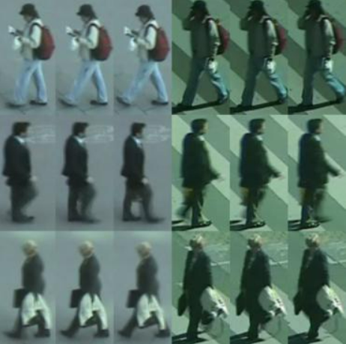
\includegraphics[width=0.5\textwidth]{images/reid_problem/prid2011.png}
    \caption{Пример изображений из набора PRID2011 \cite{hirzer2011person}}
    \label{fig:prid_2022_images_example}
\end{figure}

\section{Общая схема решения}

Общая схема работы над решением задачи \reid\ проиллюстрирована на \hyperref[fig:general_pipeline]{Рисунке \ref*{fig:general_pipeline}}. Во-первых, собираются данные с камер видеонаблюдения $-$ это исходные видео. Далее на каждом кадре размечаются \textit{\bbox}-ы $-$ прямоугольные участки изображения, в которых находятся целевые объекты. Далее каждому \bbox-у присваивается метка $-$ уникальный идентификатор человека, изображенного на кадре внутри данного \bbox-а. Теперь, когда получена разметка, следует этап обучения модели компьютерного зрения для идентификации человека по изображению. А именно, обучается нейросеть, которая строит векторные представления поступающих на вход изображений. Получаемые таким образом векторные представления используются на последнем этапе работы системы $-$ поиске соответствующего объекта в базе данных на основе близости векторных представлений.

\begin{figure}[ht]
    \centering
    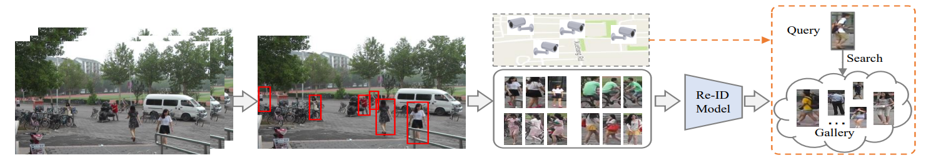
\includegraphics[width=\textwidth]{images/reid_problem/general_pipeline.png}
    \caption{Общая схема решения задачи Re-Id \cite{ye2021deep}}
    \label{fig:general_pipeline}
\end{figure}

\section{Математическая постановка задачи}

В рамках общей прикладной задачи можно выделить формальную математическую составляющую. Согласно ей, рассматриваются два множества изображений $-$ $Query$ и $Search$ (от английских названий \textit{query space} и \textit{search space} $-$ пространство запросов и пространство поиска). $Search$ представляет собой базу данных, в которой хранятся \textit{размеченные}, то есть известные изображения. Таким образом, для каждого изображения $x_j \in Search$ известна метка идентификации человека $y_j$ $-$ уникальный идентификатор, например, число в диапазоне от $1$ до $N$, где $N$ $-$ количество различных людей в базе. При этом $N \leqslant |Search|$ $-$ для каждого человека в базе может быть представлено одно или несколько изображений.

Каждый объект $q_i \in Query$ представляет собой изображение-запрос, то есть фотографию человека, личность которого неизвестна, и которую требуется установить. Для каждого $q_i$ в базе данных есть целевое множество $T_i \in Search$ $-$ множество тех картинок в базе, на которых запечатлен тот же человек. Задача состоит в том, чтобы для каждого $q_i$ выдать \textit{ранжированный список} из элементов базы, то есть перестановку $r_i \in S_{|Search|}$ из индексов в диапазоне $\overline{1, |Search|}$. Здесь $S_n$ $-$ группа всех перестановок элементов множества $\overline{1, n}$ $-$ натуральных чисел от 1 до $n$ включительно. Цель состоит в том, чтобы целевые изображения занимали позиции в начале данного списка, а изображения других людей $-$ после них. Это соответствует сортировке изображений по степени уверенности в том, что на них представлен тот же человек, что и в запросе. На \hyperref[fig:ranked_list]{Рисунке \ref*{fig:ranked_list}} представлен пример ранжированного списка. Зеленым отмечены целевые изображения, красным $-$ изображения других людей. 

Далее обсудим метрики качества решения данной задачи $-$ численные выражения соответствия действительности полученных списков.

\begin{figure}[ht]
    \centering
    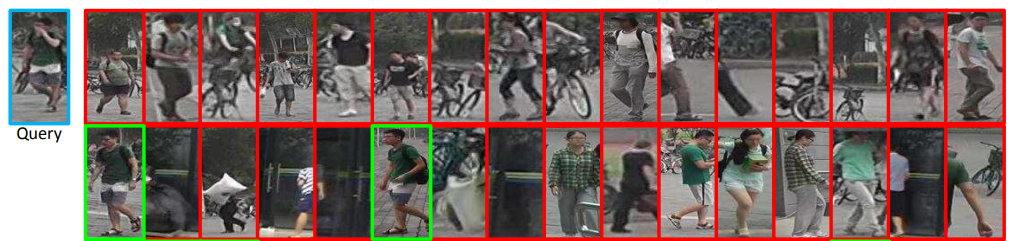
\includegraphics[width=\textwidth]{images/reid_problem/task_ranked_list.png}
    \caption{Пример ранжированного списка для одного запроса \cite{zheng2015scalable}}
    \label{fig:ranked_list}
\end{figure}

\section{Метриики качества}

\subsection{Cumulated Matching Characteristics}

Cumulated Matching Characteristics (CMC) $-$ базовый вариант оценки качества ранжированных списков. Для ее подсчета выбирается пороговое значение $-$ количество элементов от начала списка, которые берутся в рассмотрение. Для заданного порога $k$ значение метрики $CMC @ k$ определяется как доля тех запросов $q_i$, для которых среди первых $k$ элементов ранжированного списка присутствует \textit{хотя бы один} целевой объект $x_j \in T_i$:

\begin{equation}
    CMC @ k = \frac{1}{|Query|} \sum \limits_{i = 1}^{|Query|} \mathbb{I} [r_i[:k] \cap T_i \neq \varnothing].
\end{equation}

Здесь $\mathbb{I}$ $-$ индикаторная функция, $r_i[:k]$ $-$ первые $k$ элементов ранжированного списка $r_i$. Данная метрика качества в первую очередь применима в тех случаях, когда для каждого запроса в базе присутствует только один целевой объект, или, например, когда $k = 1$ $-$ при рассмотрении первого элемента списка. В случае же, если целевых объектов несколько, то при подсчете по данной формуле не учитывается порядок элементов в рассматриваемой части списка. Поэтому значение метрики будет одинаковым, независимо от того, расположен целевой объект на первых позициях или ближе к концу участка $r_i[:k]$, хотя с практической точки зрения первый вариант является более предпочтительным. Для того, чтобы преодолеть эту проблему, была введена еще одна метрика качества $-$ Mean Average Precision.

\subsection{Mean Average Precision}

Данная метрика, сокращенно $mAP$, позволяет учесть в том числе и положение целевых объектов в рассматриваемом участке ранжированного списка \cite{zheng2015scalable}. Эта метрика строится на основе стандартных метрик бинарной классификации $precision$ и $recall$: вычислется среднее значение площади под кривой Precision-Recall для всех целевых объектов. Формально, для запроса $q_i$ и каждого порога $k$ вычисляется значение

\begin{equation}
    P_i(k) = \frac{1}{k} \sum \limits_{j = 1}^{k} \mathbb I [r_i[j] \in T_i].
\end{equation}

Далее,

\begin{equation}
    AP_i = \frac{1}{|T_i|} \sum \limits_{k = 1}^{|Search|} P_i(k).
\end{equation}

И, наконец, 

\begin{equation}
    mAP = \frac{1}{|Query|} \sum \limits_{i = 1}^{|Query|} AP_i.
\end{equation}

Также применяется вариант этой метрики $-$ $mAP@k$, получаемый рассмотрением в $AP_i$ только первых $k$ элементов списка $r_i$. 

На \hyperref[fig:cmc_map]{Рисунке \ref*{fig:cmc_map}} на примере проведено сравнение CMC и mAP. Для всех трех списков значение CMC будет равно $1$, однако mAP позволяет отразить, что второй список предпочтительнее третьего.

\begin{figure}[ht]
    \centering
    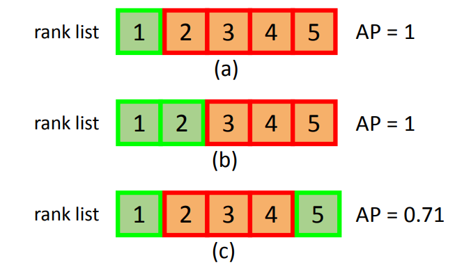
\includegraphics[width=0.5\textwidth]{images/reid_problem/metrics_example.png}
    \caption{Сравнение CMC и mAP. Для всех трех списков CMC = $1$, в то время как AP равны 1, 1 и 0.71 \cite{zheng2015scalable}}
    \label{fig:cmc_map}
\end{figure}

\section{Датасеты}

Для построения качественных систем решения задачи \reid\ существуют различные публичные датасеты, которые предоставляют большие наборы размеченных данных для обучения ML-моделей. Также они служат \textit{бенчмарками} $-$ позволяют сравнивать качество моделей на тестовой части датасета. Первые датасеты для данной задачи существуют с 2007 года. Со временем происходило увеличение датасетов $-$ как по количеству изображений, так и по количеству представленных на них людей. 

В \hyperref[tab:datasets]{Таблице \ref*{tab:datasets}} приведены характеристики основных датасетов для задачи Re-Id. Со временем в датасеты стали включаться не только размеченные вручную \bbox-ы, но и полученные автоматически с помощью ML-моделей детекции. Также некоторые датасеты включают наборы изображений-дистракторов $-$ тех кадров, которые содержат лишь фон. Включение таких изображений позволяет добиваться от системы более достоверных предсказаний, учитывающих возможность ложных срабатываний детектора людей, предоставляющего \bbox-ы. Также важно, чтобы система могла работать с изображениями разного качества, поэтому в современные датасеты включают кадры как низкого, так и высокого разрешения.

\begin{table}[]
    \centering
    \caption{Сравнение различных датасетов. Год $-$ год публикации, \#ID $-$ количество представленных людей, \#кадров $-$ общее количество изображений, \#камер $-$ количество разных камер, Размет. $-$ ручная, автоматическая или смешанная разметка \bbox-ов, Разреш. $-$ фиксированное или различное разрешение, Метрика $-$ только CMC или CMC и mAP (С \& M) \cite{ye2021deep}}
    \begin{tabular}{|l|l|l|l|l|l|l|l|}
        \hline
        \multicolumn{1}{|l|}{Датасет} & \multicolumn{1}{l|}{Год} & \multicolumn{1}{l|}{\#ID} & \multicolumn{1}{l|}{\#кадров} & \multicolumn{1}{l|}{\#камер} & \multicolumn{1}{l|}{Размет.} &
        \multicolumn{1}{l|}{Разреш.} & \multicolumn{1}{l|}{Метрика} \\ \hline
        VIPeR & 2007 & 632 & 1 264 & 2 & ручная & фикс & CMC \\ \hline
        PRID2011 & 2011 & 200 & 1 134 & 2 & ручная & фикс & CMC \\ \hline
        CUHK03 & 2014 & 1 467 & 13 164 & 2 & ручная & разн & CMC \\ \hline
        Market-1501 & 2015 & 1 501 & 32 668 & 6 & смеш & фикс & C\&M \\ \hline
        DukeMTMC & 2017 & 1 404 & 36 411 & 8 & смеш & фикс & С\&M \\ \hline
        MSMT17 & 2018 & 4 101 & 126 441 & 15 & авто & разн & С\&M \\ \hline
    \end{tabular}
    \label{tab:datasets}
\end{table}

На  \hyperref[fig:market_example]{Рисунке \ref*{fig:market_example}} приведены примеры изображений из датасета Market-1501, которые включает в себя виды с различных камер, а также изображения-дистракторы.

\begin{figure}[ht]
    \centering
    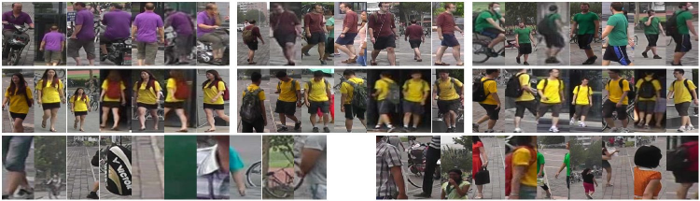
\includegraphics{images/closed_world/market_example.png}
    \caption{Пример изображений из датасета Market-1501. \cite{zheng2015scalable}}
    \label{fig:market_example}
\end{figure}



\endinput
\chapter{Подходы к решению задачи Person Re-Id}
\label{ch:closed-world}

 Общая схема построения работы системы идентификации людей содержит следующие этапы:

 \begin{enumerate}
     \item Обучение представлений признаков

     \item Метрическое обучение

     \item Оптимизация ранжирования.
    
 \end{enumerate}

 Обучение представлений признаков, или feature representation learning, $-$ это этап, на котором применяется какая-либо модель машинного обучения, позволяющая эффективно преобразовывать входное изображение в векторное представление $-$ \textit{эмбеддинг}. Данное векторное представление должно быть достаточно репрезентативным, чтобы предоставлять возможность определять по нему похожесть изображений $-$ степень уверенности в том, что на них представлен один и тот же человек. 

 Для выполнения этих требований применяются техники глубокого метрического обучения (deep metric learning). Они повзоляют построить эмбеддинги в \textit{метрическом пространстве}, то есть наделить их пространство функцией расстояния. В таком случае возникает возможность сравнивать представления изображений по их близости. Исходя из близости эмбеддингов изображений, могут быть получены ранжированние списки для изображений-запросов. Они получаются путем сортировки всех изображений из базы согласно близости их векторных представлений к эмбеддингу запроса.

 Затем, когда получены ранжированные списки, могут быть применены специальные подходы их оптимизации. Эти подходы заключаются в сравнении различных ранжированных списков между собой, для выявления более четких взаимосвязей между данными.

 Далее рассмотрим подробнее каждый этап работы системы и применяемые техники; обсудим, какие из них показывают наилучшие результаты на данный момент.


 \section{Обучение представлению признаков}

 Существует множество подходов, направленных на то, чтобы сделать эмбеддинг изображения наиболее информативным. На \hyperref[fig:feat_repr]{Рисунке \ref*{fig:feat_repr}} проиллюстрированы основные различия в этих подходах. Во-первых, базовый вариант $-$ подавать изображение напрямую в модель компьютерного зрения: сверточную сеть или трансформер, $-$ для получения итогового эмбеддинга. Во-вторых, некоторые подходы используют разделение кадра на смысловые части, позволяющее учесть локальные признаки, соответствующие, например, определенным частям тела. В-третьих, существует подходы, которые прибегают к вспомогательной информации для наделения эмбеддинга изображения дополнительными свойствами. И, наконец, часть подходов опирается на тот факт, что все кадры, содержащие целевой объект, поступают на вход системы из видеозаписи, что позволяет обрабатывать их как упорядоченную последовательность и моделировать более состоятельные закономерности.

 \begin{figure}[ht]
     \centering
     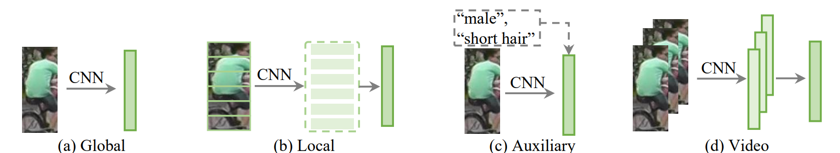
\includegraphics{images/closed_world/feat_repr_learning.png}
     \caption{Варианты работы системы на этапе обучения представлению признаков \cite{ye2021deep}}
     \label{fig:feat_repr}
 \end{figure}

 \subsection{Глобальное представление признаков}

 Данный вариант представляет собой применение, или \textit{инференс}, нейросети компьютерного зрения на изображении целиком. Так, сверточная сеть, преобразует входной кадр на каждом слое в карту признаков, из которой в итоге формируется один эмбеддинг. В базовом случае этот процесс применяется к каждому изображению датасета в режиме \textit{single-image}, то есть независимо. Однако существуют методы, которые принимают на вход пары изображений, что соответствует режиму \textit{cross-image} \cite{wang2016joint}. В таком случае карты признаков обоих изображений подаются вместе в модель построения итогового эмбеддинга, как показано на \hyperref[fig:cross_image]{Рисунке \ref*{fig:cross_image}}. Таким образом система работает в режиме верификации $-$ определения того, соответствуют два изображения одному и тому же человеку или нет.

 \begin{figure}[ht]
     \centering
     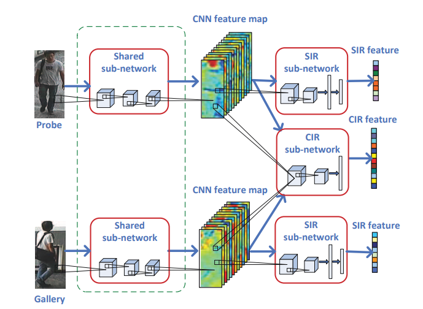
\includegraphics[width=0.7\textwidth]{images/closed_world/single_cross_image.png}
     \caption{Single-image и Cross-image режимы \cite{wang2016joint}}
     \label{fig:cross_image}
 \end{figure}

 \subsection{Локальное представление признаков}

 Методы этого типа раскладывают входное изображение на несколько пространственных составляющих, отвечающих различным \textit{регионам интереса}. Во-первых, регионы интереса могут соответствовать частям тела и использовать отдельную модель детекции для определения их местоположения \cite{suh2018part}, как показано на \hyperref[fig:body_part]{Рисунке \ref*{fig:body_part}}.

 \begin{figure}[ht]
     \centering
     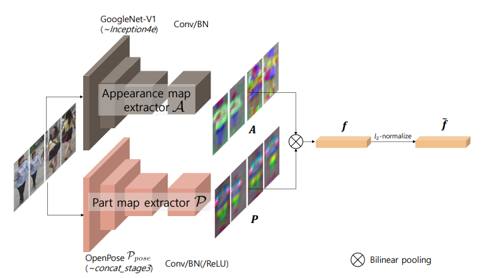
\includegraphics[width=0.7\textwidth]{images/closed_world/body_part_detection.png}
     \caption{Извлечение локальных признаков с помощью детекции частей тела \cite{suh2018part}}
     \label{fig:body_part}
 \end{figure}

 Во-вторых, некоторые методы \cite{su2018beyond} обрабатывают регионы интереса как отдельные изображения, что позволяет параллельно извлечь из кадра информацию разного типа. При этом регионы могут быть получены исходя из детекции частей тела, ключевых точек или же из нарезки изображения на равные слои по вертикали или по горизонтали (см. \hyperref[fig:image_slicing]{Рисунок \ref*{fig:image_slicing}}).

 \begin{figure}[ht]
     \centering
     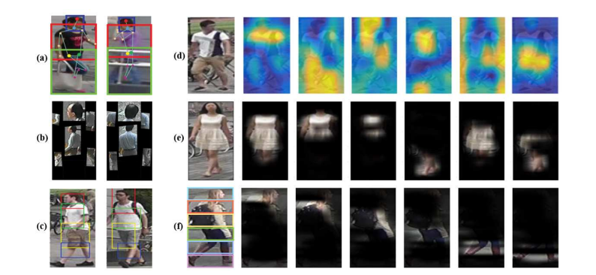
\includegraphics[width=0.7\textwidth]{images/closed_world/image_slicing.png}
     \caption{Нарезка изображения на части \cite{su2018beyond}}
     \label{fig:image_slicing}
 \end{figure}

 \subsection{Использование дополнительной информации}

 Наибольший научный интерес в рамках данной работы представляют методы, прибегающие к вспомогательной информации для построения информативного эмбеддинга изображения человека. 

 Одна группа таких методов опирается на семантические атрибуты $-$ текстовые описания или же метки классификации \cite{lin2019improving}, \hyperref[fig:semantic_attributes]{Рисунок \ref*{fig:semantic_attributes}}. Действительно, каждый человек в рамках данной задачи может быть классифицирован по таким категориям, как пол, возраст, цвет и длина волос, тип и цвет одежды и др. Информация об этой классификации может подаваться в модель в разном виде. Она может подаваться на вход, может сроиться отдельный эмбеддинг модели классификации. Также с помощью дополнительной инфорации может строиться фильтрация релевантных/не-релевантных объектов. Кроме того, могут применяться метрические методы для установления соответствия между эмбеддингом атрибутной информации и основным эмбеддингом изображения.

 \begin{figure}[ht]
     \centering
     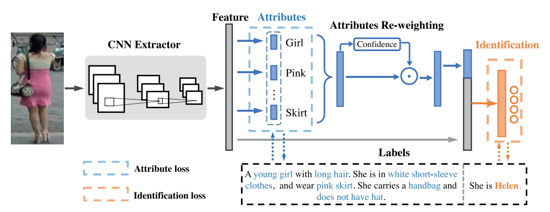
\includegraphics[width=0.7\textwidth]{images/closed_world/semantic_attributes.png}
     \caption{Использование семантических атрибутов \cite{lin2019improving}}
     \label{fig:semantic_attributes}
 \end{figure}

 Также существует методы, рассматривающие изображения с каждой камеры как отдельный домен, то есть однородную часть в неоднородном общем датасете \cite{liu2019view}, \hyperref[fig:viewpoint_information]{Рисунок \ref*{fig:viewpoint_information}}.

 \begin{figure}[ht]
     \centering
     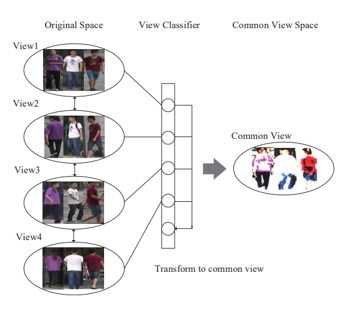
\includegraphics[width=0.5\textwidth]{images/closed_world/viewpoint_information.png}
     \caption{Кросс-доменная идентификация для кадров с различных камер \cite{liu2019view}}
     \label{fig:viewpoint_information}
 \end{figure}

 В такой постановке применяются технологии кросс-доменной идентификации, направленные на построения таких представлений изображений, которые обладают инвариантностью к смене домена. Так, например, один из методов включает в функцию потерь ограничение на близость между матрицами корреляций признаков изображений из разных доменов \cite{lin2017consistent}, \hyperref[fig:domain_information]{Рисунок \ref*{fig:domain_information}}.

 \begin{figure}[ht]
     \centering
     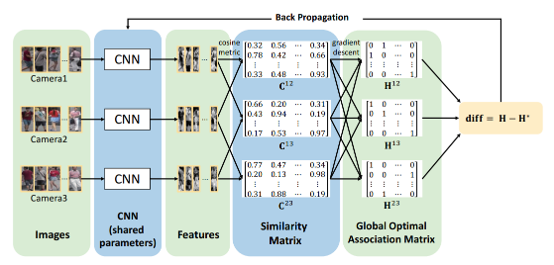
\includegraphics[width=0.7\textwidth]{images/closed_world/domain_information.png}
     \caption{Использование доменной информации \cite{lin2017consistent}}
     \label{fig:domain_information}
 \end{figure}

 Еще одной из важных техник, затрагивающей дополнительную информацию, является аугментация датасетов, в том числе с помощью генеративных моделей \cite{zheng2017unlabeled}. Общий план такого метода, как показано на \hyperref[fig:dataset_augmentation]{Рисунке \ref*{fig:dataset_augmentation}}, состоит в том, чтобы дополнить датасет данными для тех объектов, для которых мало размеченных примеров, и использовать полученные синтетические данные при обучения модели.

 \begin{figure}[ht]
     \centering
     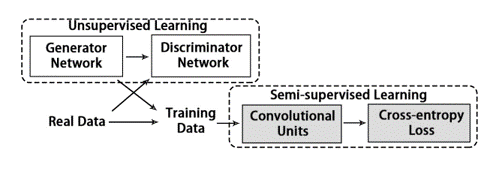
\includegraphics[width=0.5\textwidth]{images/closed_world/dataset_augmentation.png}
     \caption{Аугментация датасета с помощью генеративных моделей \cite{zheng2017unlabeled}}
     \label{fig:dataset_augmentation}
 \end{figure}

 \subsection{Идентификация на видео}

 Наконец, еще один способ промоделировать общие закономерности данных заключается в том, чтобы подавать кадры видеозаписей не по-отдельности, а в виде упорядоченной последовательности, что иллюстрирует \hyperref[fig:rnn]{Рисунок \ref*{fig:rnn}}. В таком случае применимы различные методы обработки последовательных данных, такие как рекуррентные сети и трансформеры \cite{haque2016recurrent}.

 \begin{figure}[ht]
     \centering
     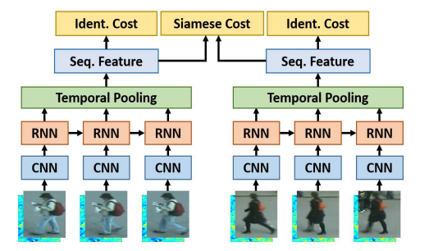
\includegraphics[width=0.5\textwidth]{images/closed_world/rnn.png}
     \caption{Применение моделей обработки последовательностей для видео \cite{haque2016recurrent}}
     \label{fig:rnn}
 \end{figure}



 \section{Метрическое обучение}

 Ключевая часть в построении системы, решающей задачу \reid\ $-$ это метрическое обучение, или \textit{metric learning}. Его суть состоит в том, чтобы с помощью функции потерь учесть тот факт, что эмбеддинги должны лежать в метрическом пространстве. Таким образом, эмбеддинги кадров, соответствующих одному и тому же человеку, должны лежать близко к друг другу, а между изображениями разных людей расстояние должно быть большим. В такой постановке возникает два важных аспекта работы $-$ дизайн самой лосс-функции и построение хода обучения таким образом, чтобы на каждой итерации модель с помощью этой лосс-функции усваивала наиболее важные закономерности в данных.

 \subsection{Дизайн функции потерь}

 \textbf{Softmax loss}. Базовый вариант $-$ обучение модели на решение задачи классификации. В таком случае каждый класс $-$ это один человек, представленный в датасете, и модель обучается отличать их друг от друга, используя softmax loss, или же identity loss, \hyperref[fig:identity_loss]{Рисунок \ref*{fig:identity_loss}}:

 \begin{figure}[ht]
     \centering
     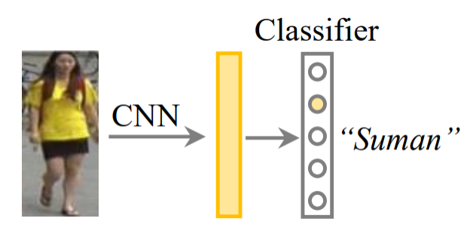
\includegraphics[width=0.5\textwidth]{images/closed_world/identity_loss.png}
     \caption{Лосс-функция идентификации \cite{ye2021deep}}
     \label{fig:identity_loss}
 \end{figure}

 \begin{equation}
     \mathcal L_{S} = \mathcal L_{id} = - \frac{1}{n}\sum \limits_{i = 1}^n \log \left( p (y_i | x_i) \right) = \frac{1}{n}\sum \limits_{i = 1}^n \log \frac{e^{W_{y_i}^T x_i + b_{y_i}}}{\sum_{j=1}^m e^{W_j^T x_i + b_j}}.
 \end{equation}

 Здесь $n$ $-$ количество объектов в батче, $m = |Search|$ $-$ количество классов, то есть различных людей в датасете, $x_i$ $-$ эмбеддинг $i$-того объекта, $W_j$ и $b_j$ $-$ вес и свободный член классификатора, соответстующие данному классу $j$.

 Недостаток этого метода состоит в том, что нет гарантий для применимости этого метода для неизвестных объектов, поскольку свойство метрического пространства не закладывается в модель.

 \textbf{Center loss}. Один из вариантов наделения пространства эмбеддингов информативной метрикой $-$ кластеризация \cite{wen2016discriminative}, \hyperref[fig:center_loss]{Рисунок \ref*{fig:center_loss}}. Так, подход center loss заключается в том, чтобы добавить слагаемое, отвечающее за разделение эмбеддингов разных классов на кластеры:

 \begin{figure}[ht]
     \centering
     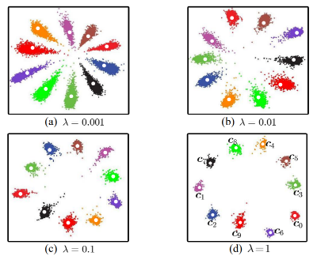
\includegraphics[width=0.5\textwidth]{images/closed_world/center_loss.png}
     \caption{Кластеризация с помощью center loss \cite{wen2016discriminative}}
     \label{fig:center_loss}
 \end{figure}

 \begin{equation}
     \mathcal L_{C} = - \frac{1}{2}\sum \limits_{i = 1}^n  \| x_i - c_{y_i} \|^2,
 \end{equation}
 \begin{equation}
     \mathcal L = \mathcal L_S + \lambda \mathcal L_C.
 \end{equation}

 \textbf{Binary verification loss}. В этом подходе изображения подаются в нейросеть парами. Для обоих изображений модель строить свой эмбеддинг, и затем эта пара эмбеддингов подается в итоговый бинарный классификатор: один и тот же это объект или нет \cite{li2014deepreid}, \hyperref[fig:binary_verification_loss]{Рисунок \ref*{fig:binary_verification_loss}}.

 \begin{figure}[ht]
     \centering
     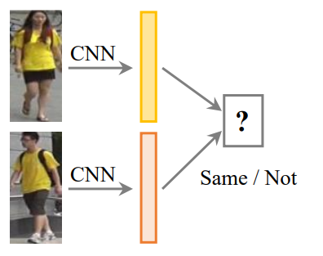
\includegraphics[width=0.5\textwidth]{images/closed_world/binary_verification_loss.png}
     \caption{Лосс-функция верификации \cite{li2014deepreid}, \cite{ye2021deep}}
     \label{fig:binary_verification_loss}
 \end{figure}

 \begin{equation}
     \mathcal L_{very}(i, j) = - \delta_{ij} \log \left( p(\delta_{ij} | x_{ij}) \right) - (1 - \delta_{ij}) \log \left( 1 - p(\delta_{ij} | x_{ij}) \right).
 \end{equation}

 Здесь $\delta_{ij}$ $-$ индикатор того, что кадры $i$ и $j$ представляют один объект, $x_{ij}$ $-$ их совместное представление. Недостаток этого метода состоит в том, что необходимо подавать изображения парами, следовательно, для поиска целевого объекта нужно перебрать все изображения из базы.

 \textbf{Contrastive loss}. В данном варианте можно подавать изображения в модель как парами, так и независимо. Лосс-функция накладывает на эмбеддинги свойства метрического пространства, пропорционально штрафуя модель за близкие по метрике $d$ представления изображений разных объектов и далекие представления разных \cite{hadsell2006dimensionality}. При этом используется пороговое значение отступа $\rho$, которое принимается достаточным для разделения объектов; выше этого значения штраф не назначается:

 \begin{equation}
     \mathcal L_{con} = (1 - \delta_{ij}) \{ \max (0, \rho - d_{ij}) \}^2 + \delta_{ij} d_{ij}^2.
 \end{equation}

 \textbf{Triplet loss}. Один из наиболее распространеных и эффективных методов является использование triplet loss-а \cite{schroff2015facenet}. Этот способ позволяет промоделировать более широкие взаимосвязи между данными. Изображения объединяются в тройки, содержащие опорный, или \textit{якорный}, объект, а также \textit{позитивный} и \textit{негативный} примеры. Позитивный пример соответствует тому же человеку, что и якорный, а негативный $-$ другому. Цель состоит в том, чтобы на очередном шаге оптимизации приблизить к опорному объекту $i$ позитивный пример $j$ и отдалить негативный $k$, \hyperref[fig:triplet_loss]{Рисунок \ref*{fig:triplet_loss}}.

 \begin{figure}[ht]
     \centering
     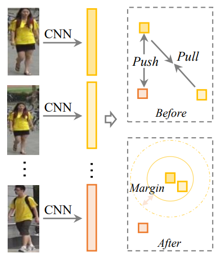
\includegraphics[width=0.5\textwidth]{images/closed_world/triplet_loss.png}
     \caption{Triplet loss \cite{schroff2015facenet}, \cite{ye2021deep}}
     \label{fig:triplet_loss}
 \end{figure}

 \begin{equation}
     \mathcal L_{tri} (i, j ,k) = \max \left( \rho + d_{ij} - d_{ik}, 0 \right).
 \end{equation}

 \textbf{SphereFace}. Этот метод представляет собой развитие softmax loss-а. Его суть в том, чтобы расположить эмбеддинги в метрическом пространстве на многомерное сфере, как показано на \hyperref[fig:sphereface]{Рисунке \ref*{fig:sphereface}}, и относить к определенному классу исходя не из аффинной проекции, а из угла между эмбеддингом и весом классификатора, соответствующим данному классу \cite{liu2017sphereface}.

 \begin{figure}[ht]
     \centering
     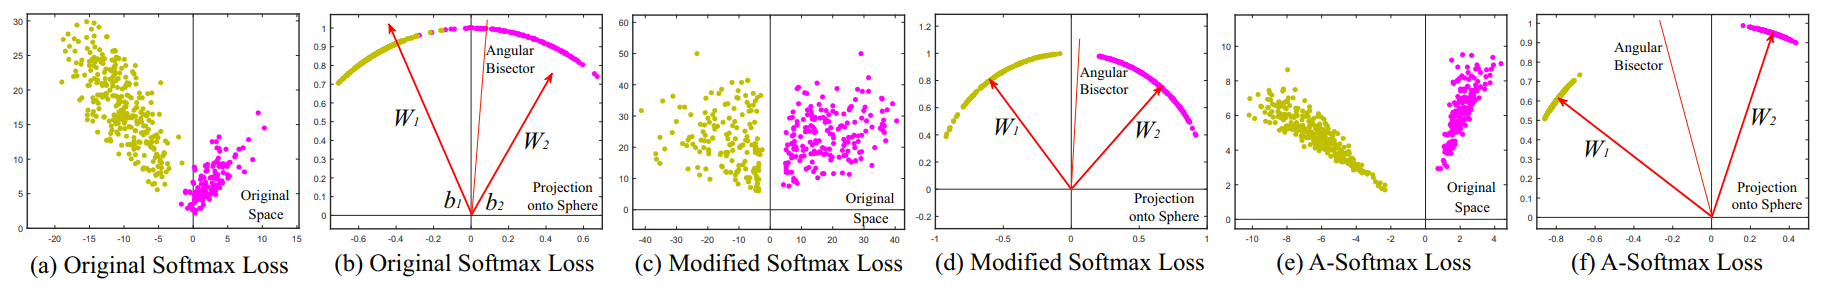
\includegraphics{images/closed_world/sphereface_whole.png}
     \caption{Функция потерь SphereFace сравнивает эмбеддинги по углу с вектором параметров классификатора \cite{liu2017sphereface}}
     \label{fig:sphereface}
 \end{figure}

 \begin{equation}
     \mathcal L_{modified} = - \frac{1}{n} \sum \limits_{i = 1}^{n} \log \frac{e^{\|x_i\| \cos (\theta_{y_i, i}) }}{e^{\|x_i\| \cos (\theta_{y_i, i})} + \sum_{j \neq y_i} e^{\|x_i\| \cos (\theta_{j, i})}}
 \end{equation}

 \begin{equation}
     \mathcal L_{ang} = - \frac{1}{n} \sum \limits_{i = 1}^{n} \log \frac{e^{\|x_i\| \psi (\theta_{y_i, i}) }}{e^{\|x_i\| \psi (\theta_{y_i, i})} + \sum_{j \neq y_i} e^{\|x_i\| \cos (\theta_{j, i})}}
 \end{equation}

 \textbf{CosFace, ArcFace}. Наконец, продолжая предыдущий метод, функции CosFace и ArcFace вводят в функцию потерь отступ, позволяющий разделять классы с некоторым зазором. Оптимальным вариантом является разделение прямой полосой с сферических координитах, что иллюстрирует \hyperref[fig:arcface]{Рисунке \ref*{fig:arcface}}.

 \begin{figure}[ht]
     \centering
     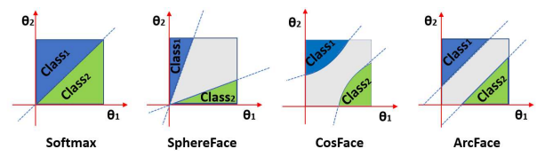
\includegraphics{images/closed_world/arcface.png}
     \caption{Функции CosFace и ArcFace позволяют строить зазор между эмбеддингами на сфере \cite{wang2018cosface}, \cite{deng2019arcface}}
     \label{fig:arcface}
 \end{figure}

 \begin{equation}
     \mathcal L_{cos} = - \frac{1}{n} \sum \limits_{i = 1}^{n} \log \frac{e^{s \left(  \cos (\theta_{y_i, i}) - m \right)}}{e^{s \left(  \cos (\theta_{y_i, i}) - m \right)} + \sum_{j \neq y_i} e^{s \cos (\theta_{j, i})}}
 \end{equation}

 \begin{equation}
     \mathcal L_{arc} = - \frac{1}{n} \sum \limits_{i = 1}^{n} \log \frac{e^{s \left(  \cos (\theta_{y_i, i} + m) \right)}}{e^{s \left(  \cos (\theta_{y_i, i} + m) \right)} + \sum_{j \neq y_i} e^{s \cos (\theta_{j, i})}}
 \end{equation}

 \subsection{Процесс обучения}

 Для некторых из представленных функций, в частности, для триплет-лосса, важной задачей является также подбор на каждой оптимизационной итерации наиболее сложных семплов датасета, обучение на которых внесет наибольший вклад в наполнение моделью информации о данных. Так, распространена техника \textit{hard-batch triplet mining} $-$ в качестве позитивного примера подается целевой кадр из батча, содержащий тот же объект, и представление которого наиболее отдалено от представления якорного. Аналогично, в качестве негативного подается наиболее близкий из остальных кадров. Кроме того, существуют техники, позволяющие моделировать более широкие взаимосвязи в данных для выявления оптимальных триплетов. Так, например, работа \cite{zeng2020hierarchical} объединяет метод hard-batch с иерархической кластеризацией семплов для выявления оптимальных троек кадров, \hyperref[fig:clusters]{Рисунок \ref*{fig:clusters}}:

 \begin{figure}[ht]
     \centering
     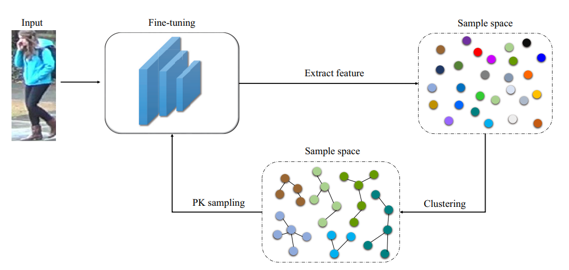
\includegraphics[width=0.7\textwidth]{images/closed_world/clusters.png}
     \caption{Иерархическая кластеризация в связке с hard-batch триплет mining \cite{zeng2020hierarchical}}
     \label{fig:clusters}
 \end{figure}


 \section{Оптимизация ранжирования}

 Благодаря метрическому обучению возможно получение ранжированных списков для объектов, поскольку функция расстояния позволяет упорядочить изображения в соответствии с похожестью. Однако данные списки могут быть улучшены, с помощью учета о взаимном положении объектов в ранжированных списках друг друга. Можно выделить две основные техники.

 \textbf{Ре-ранкинг}. Этот способ основан на том, что если два кадра соответствуют одному и тому же человеку, то каждый из них должен присутствовать в начале ранжированного списка другого. Поэтому данный метод позволяет удалить из списков некоторые неправильные ответы и добавить изначально ненайденные. Рассмотрим процедуру $k$-\textit{reciprocal re-ranking} \cite{zhong2017re}, проиллюстрированную на \hyperref[fig:reranking]{Рисунке \ref*{fig:reranking}}. На первом шаге для каждого кадра $x$ в ранжированном списке $r$ запроса $q$, имеющем размер $k$, строится свой ранжированный список размера $k$. Если $q$ в нем отсутствует, то $x$ удаляется из списка $r$. На втором шаге список $r$ пополняется константным количеством объектов из списков каждого оставшегося в $r$ кадра. Данная операция удаления-пополнения приводит к сокращению числа как ложно-положительных, так и ложно-отрицательных ответов.

 \begin{figure}[ht]
     \centering
     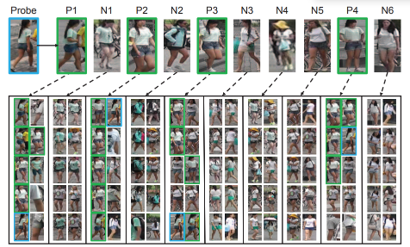
\includegraphics[width=0.7\textwidth]{images/closed_world/reranking.png}
     \caption{k-reciprocal re-ranking \cite{zhong2017re}}
     \label{fig:reranking}
 \end{figure}

 Полученные после этого алгоритма списки могут быть сравнены с помощью функции \textit{расстояния Джакарда}, которая строится на основе отношения размеров пересечения и объединения двух списков:

 \begin{equation}
     \mathcal R (q_i, k) = \{ x_j | (x \in r_i[:k]) \wedge (q \in r_j[:k]) \}
 \end{equation}

 \begin{equation}
     d_{J} (q_i, x_j) = 1 - \frac{| R(q_i, k) \cap R(x_j, k) |}{| R(q_i, k) \cup R(x_j, k)  |}
 \end{equation}

 \textbf{Слияние ранжированных списков}. Данный подход представляет собой метод ансамблирования нескольких моделей. Работа \cite{ye2016person} предлагает подход объединения ранжированных списков, основанный на усилении соотношений похожести между объектами в началах списков и непохожести $-$ в концах, \hyperref[fig:rank_fusion]{Рисунок \ref*{fig:rank_fusion}}:

 \begin{figure}[ht]
     \centering
     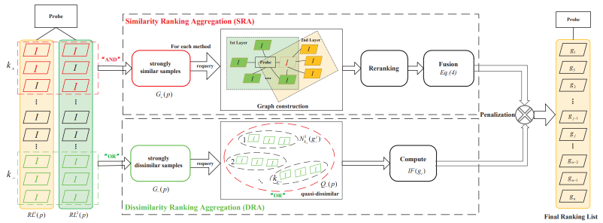
\includegraphics[width=0.7\textwidth]{images/closed_world/rank_fusion.png}
     \caption{Слияние ранжированных списков \cite{ye2016person}}
     \label{fig:rank_fusion}
 \end{figure}



 \endinput
\chapter{Сферы применения технологий Re-Id}
\label{ch:applications}

Обсудим основные сферы применения технологий \reid. Как упоминалось выше, большинство методов способны обрабатывать данные совершенно разных предметных областей, или \textit{доменов}. Действительно, основные техники, применяемые в задаче Re-Id, такие как метрическое обучение, оптимизация ранжирования, использование дополнительной информации, аугментации, работа с видео-последовательностью, могут быть распространены и на другие домены. В то же время часть методов, таких как детекция частей тела, нарезка изображения на части, обучение локальных признаков, либо не могут быть перенесены на данные другой предметной области, либо должны быть преобразованы. Таким образом, различные сферы применения Re-Id технологий, перечисленные ниже, объединены общей постановкой задачи и структурой работы системы, однако каждая из них содержит свои нюансы.

\section{Распознавание по лицу для контроля доступа}

В современном мире широкую популярность имеют технологии \textit{Face-ID}, позволяющие производить идентификацию по фотографии лица человека. Во-первых, они используются для аутентификации пользователя в компьютерах, смартфонах и других устройствах. Во-вторых, те же технологии применяются для работы систем оплаты \textit{face-pay} в транспорте и магазинах. Кроме этого, техники идентификации по лицу могут быть встроены в сложные многоуровневые системы доступа к системам повышенной безопасности.


\section{Идентификация людей для обеспечения безопасности}

В данном случае речь идет об обнаружении подозрительных личностей, или же конкретных людей, которые могут быть вовлечены в противоправную деятельность. Данный вариант применения технологии наиболее акутален для предприятий, в том числе секретных, а также для общественных учреждений с высоким скоплением людей. Также к этой сфере применения относится отслеживание перемещения подозреваемого человека между разными локациями, в которых установлены камеры видеонаблюдения. Технологии ре-идентификации позволяют строить траекторию движения конкретного человека, исходя из видео-данных с этих камер.


\section{Отслеживание транспортных средств}

Еще одной важной сферой применения технологий \reid\ является мониторинг движения автомобилей. Одной из задач в этой области является построение траектории движения конкретного автомобиля на дороге для контроля соблюдения ПДД: соблюдение скоростного режима, разметки полос, правил обгона и др. В таком случае методы Re-ID сочетаются с другими техниками компьютерного зрения. Во-первых, для построения траектории движения применяются в том числе техники \textit{трекинга}, то есть объединения информации о положении объекта на различных последовательных кадрах, основанных на последовательном вычислении и обновлении значений его скорости и направления в пространстве. Однако для улучшения построения траекторий, в частности, в условиях пересечения траекторий нескольких разных объектов, применимы в том числе технологии ре-идентификации, позволяющие правильно совместить продолжения траекторий объектов после их расхождения. Во-вторых, на этапе ре-идентификации используется также дополнительная информация о государственных номерах автомобилей, получаемая смежными методами компьютерного зрения. Таким образом, данный домен данных содержит общие черты с задачей \reid, а также некоторые уникальные особенности.


\section{Розничная торговля}

Здесь речь идет о нескольких путях применения ре-идентификации. Так, они могут быть использованы для анализа перемещений клиентов на территории магазина или торгового центра с помощью сопоставления их изображений на данных разных камер и построения общей траектории.

Кроме того, методы Re-Id применяются также для оптимизации контроля наличия товаров на прилавках. В данном случае задача сочетается с базовой постановкой классификации в компьютерном зрении, но не сводится к ней. Действительно, для корректной работы такой системы необходимо обрабатывать в том числе те объекты, для которых в данных имеется мало обучающих примеров, а также неизвестные объекты, в случае изменения ассортимента. Кроме того, в этой сфере применимы также технологии использования вспомогательной информации, такие как, например, наименования товаров или их текстовые описания.


\section{Поиск пропавших домашних животных}

Одной из основных сфер применения ре-идентификации, рассматриваемых в данной работе, является система поиска пропавших собак по данным городских камер видеонаблюдения. Данная система реализована в процессе выполнения бакалаврской работы. Рассмотрим подробно устройство этой системы в следующем разделе.



\endinput
\chapter{Система поиска пропавших домашних животных}
\label{ch:petsearch}

Система поиска пропавших домашних животных, реализованная в рамках проекта компании ООО "НКБТех"\ и в процессе выполнения данной бакалаврской работы, ставит свой целью отслеживание их передвижений в областях видимости различных городских камер видеонаблюдения. Для этого используется пайплайн из нескольких технологий компьютерного зрения и анализа данных, схема которого представлена на \hyperref[fig:petsearch_scheme]{Рисунке \ref*{fig:petsearch_scheme}}:

\begin{figure}[ht]
	\centering
	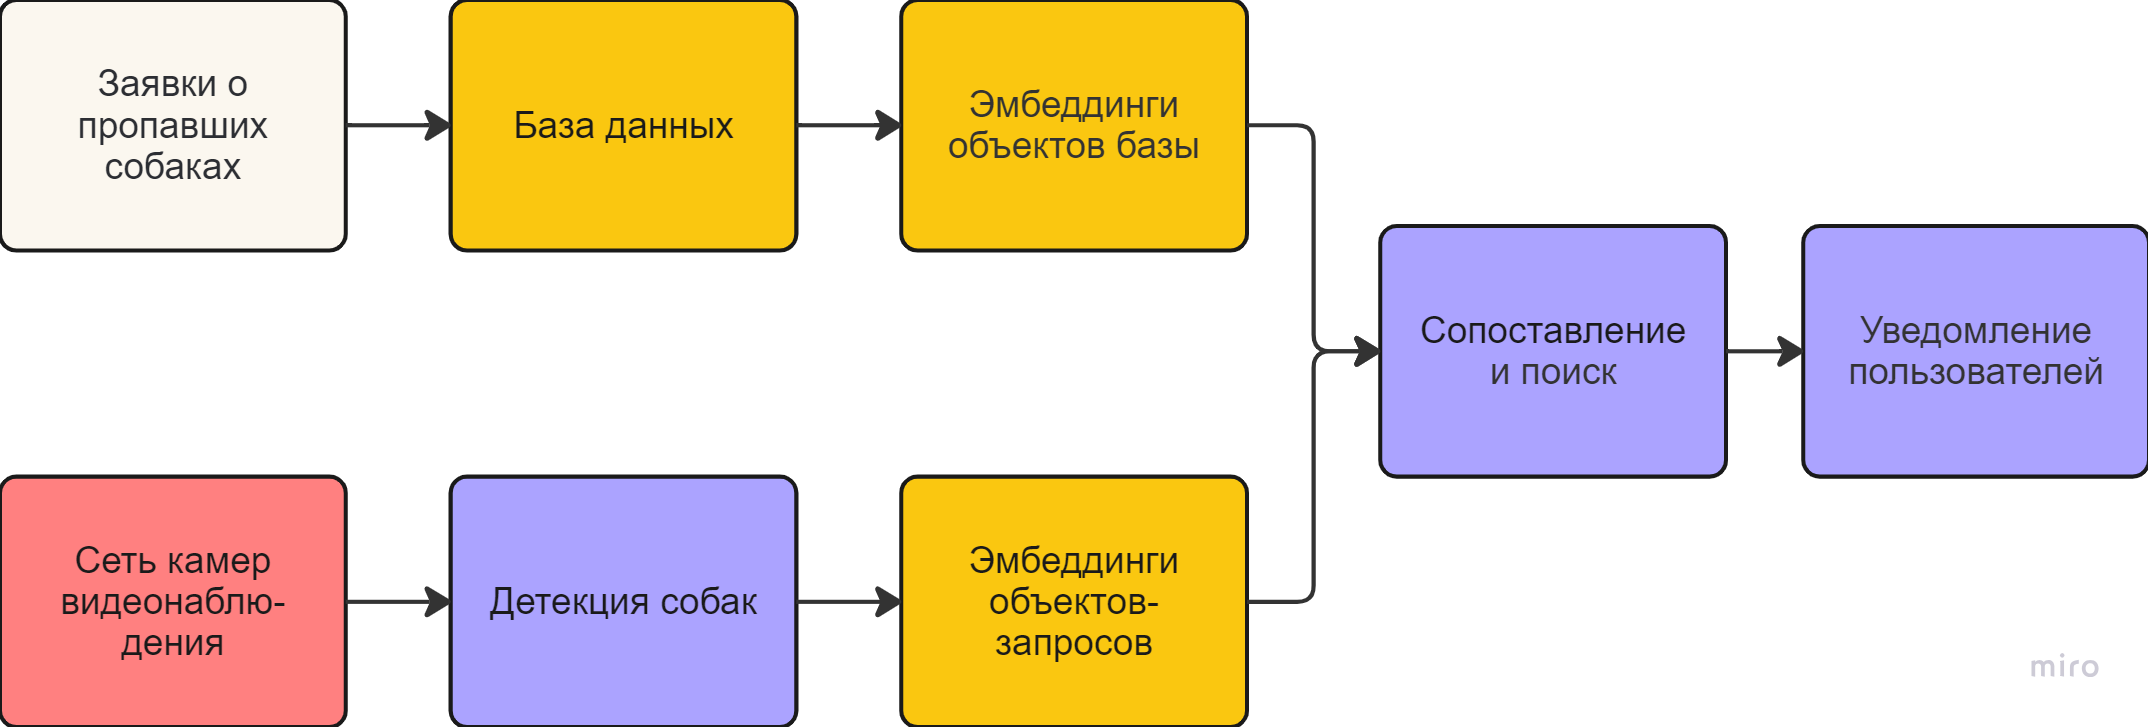
\includegraphics[width=0.9\textwidth]{images/petsearch/scheme.png}
	\caption{Схема работы системы поиска}
	\label{fig:petsearch_scheme}
\end{figure}

\begin{enumerate}
    \item Создание базы данных разыскиваемых животных

    \item Подключение городской системы видеонаблюдения к базе данных

    \item Детекция животных на видео

    \item Идентификация обнаруженного объекта с помощью техник Re-Id

    \item Поиск соответствий в базе данных

    \item Построение траектории движения в реальном времени

\end{enumerate}

На первом этапе формируется база данных из потерявшихся животных. В нее заносятся записи от пользователей, содержащие одну или несколько фотографий их питомца. Кроме этого, может быть предоставлена дополнительная информация в виде текстового описания, а также классификация по некоторым важным категориям. На текущем этапе развития проекта в качестве питомцев рассматриваются только собаки, соответственно, признаки классификации выбраны специфичными именно для них. Согласно Российской кинологической федерации, наиболее информативными признаками для описания собак являются цвет, размер, длина лап относительно туловища, длина морды, форма ушей и тип шерсти. В дальнейшем поиск производится на основе всей имеющейся информации.

Далее выполняется подключение к камерам городского видеонаблюдения. Суммарно на данном этапе реализации проекта доступно несколько сотен камер в пределах одного района. 

Затем сервис обработки видеопотока подает кадры с камер в модель компьютерного зрения для детекции объектов. Среди результатов детекции отбираются те, которые соответствуют классу "собака".

После этого каждый обнаруженный \bbox, содержащий собаку, с помощью Re-Id модели переводится в эмбеддинг, который затем сравнивается с эмбеддингами изображений из базы данных. Также с помощью отдельной модели может быть произведена классификация для фильтрации по соответствию основных признаков. Также с помощью мультимодальных моделей, таких как CLIP \cite{radford2021learning} и CLIP-ReID \cite{li2023clip} может быть построено соответствие текстовому описанию. Исходя из метрической близости эмбеддингов находятся соответствия с объектами базы. Таким образом, отбирается одна или несколько записей, которые соответствуют обнаруженной в данной момент собаке, и соответствующим пользователям присылаются уведомления об обнаружении животного.

Наконец, поскольку обработка видеопотока, детекция и поиск происходят в режиме реального времени, возможно построение траектории движения обнаруженной собаки между областями обзора камер, следуя которой можно достичь местоположения животного.


\section{Датасеты}

Существует несколько публичных датасетов, посвященных методам обработки изображений животных. Основные датасеты, сфокусированные на изображениях собак $-$ Tsinghua Dog \cite{Zou2020ThuDogs} и Stanford Dog \cite{khosla2011novel}. Они содержат разметку на породы собак, включающую в себя большое количество категорий и подкатегорий.

Однако с точки зрения системы поиска классификация по породам не всегда является оптимальной. Так, собаки одной и той же породы могут иметь разный цвет, или же разные комбинации цветов, и в таком случае именно дифференциация по цвету будет являться более информативной. Также собаки некоторых пород, например, пуделей, встречаются как больших размеров, так и карликовые.

В связи с этим в рамках разработки проекта компанией был собран собственный датасет классификации собак. Он включает в себя $50\ 000$ изображений собак с выставки и разметку для 6 категорий. Пример изображений из датасета можно увидеть на \hyperref[fig:petsearch_dataset]{Рисунке \ref*{fig:petsearch_dataset}}. Изображения собак представляют собой фотографии с выставки, обработанные с помощью выделения \bbox-ов, содержащих собак, благодаря чему наблюдается высокая репрезентативность как по породам, так и по классификационным признакам. В \hyperref[tab:datasets_dog]{Таблице \ref*{tab:datasets_dog}} приведены описания признаков классификации.

\begin{figure}[ht]
	\centering
	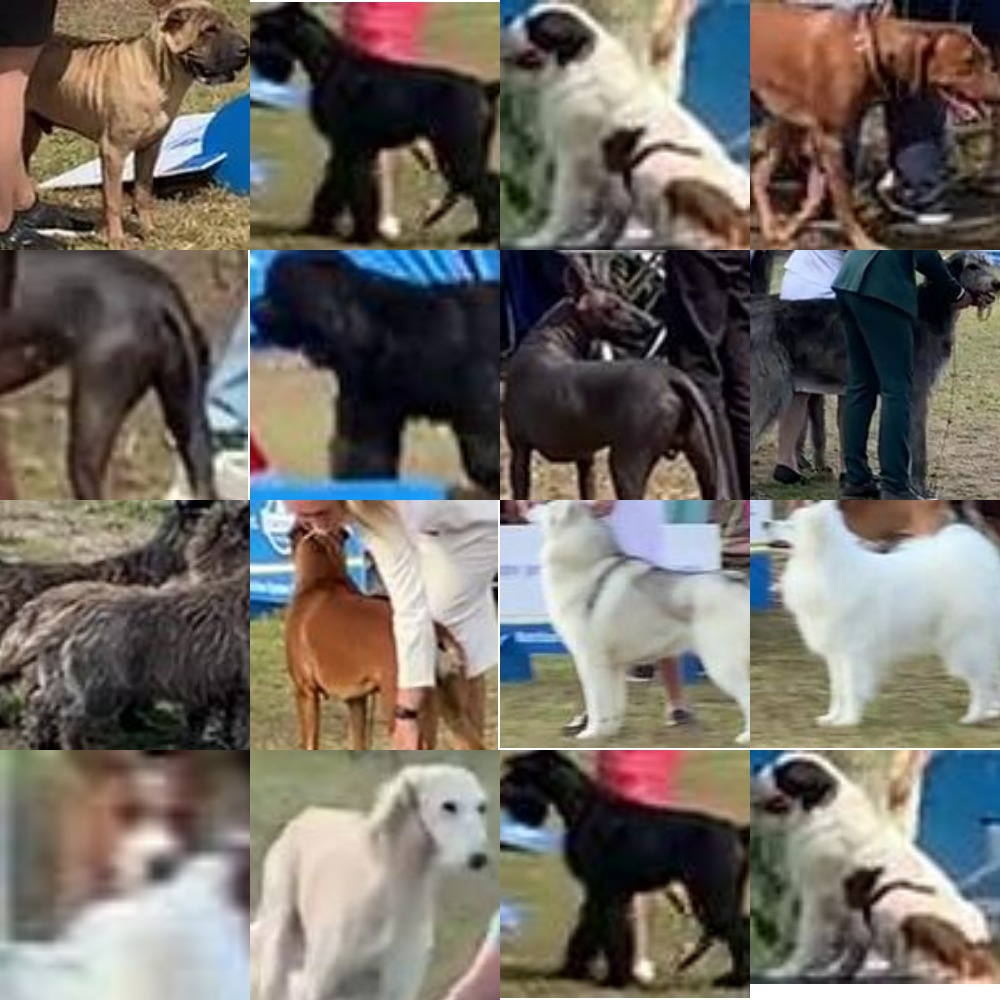
\includegraphics[width=0.7\textwidth]{images/petsearch/dataset.jpg}
	\caption{Пример изображений из датасета}
	\label{fig:petsearch_dataset}
\end{figure}

\begin{table}[]
    \centering
    \caption{Категории классификации в датасете}
    \begin{tabular}{|l|l|l|}
        \hline
        \multicolumn{1}{|l|}{Признак} & \multicolumn{1}{l|}{Количество значений} & 
        \multicolumn{1}{l|}{Значения}\\ \hline
        Цвет & 11 & белый, бежевый, \\ & & черно-белый, черно-рыже-белый, \\ & & черно-рыжий, черно-серый, \\ & & черный, серый, \\ & & рыжий, коричневый, \\ & & коричнево-белый \\ \hline
        Размер & 3 & большой, средний, малый \\ \hline
        Длина лап & 2 & длинные, короткие \\ \hline
        Тип ушей & 3 & стоячие, полу-висячие, \\ & & стоячие \\ \hline
        Тип морды & 2 & длинная, короткая \\ \hline
        Тип шерсти & 5 & длинношерстный, среднешерстный, \\ & & гладкошерстный, безшерстный, \\ & & курчавый \\ \hline
    \end{tabular}
    \label{tab:datasets_dog}
\end{table}

К сожалению, ни один из датасетов не предоставляет разметки напрямую для задачи Re-Id. Таким образом, измерить качество решения данной задачи можно лишь косвенно, то есть на основе вспомогательной информации, опираясь на качество решения задачи классификации или с помощью визуальной оценки ранжированных списков.


\section{Решение с помощью классификации}

Таким образом, в данной постановке возможно решить задачу классификации объектов. Для классификации собак по породам существуют решения, имеющие качество, близкое к $100 \%$ \cite{bera2022sr}. Однако классификация по специфичным признакам, представленным в нашем датасете, является более сложной задачей и на данный момент не имеет решения с высоким качеством.

В рамках исследования были проведены эксперименты по обучения ML-моделей для классификации собак. Процесс обучения строился в двух вариантах: в первом варианте для каждого признака обучалась своя модель, а во втором обучалась одна модель с шестью классификаторами на выходе. Оба способа показали схожее качество. Репозиторий с кодом, использованным для проведения экспериментов, доступен по ссылке: \href{https://github.com/nkb-tech/nkb-classification}{https://github.com/nkb-tech/nkb-classification}.

Были проверены различные архитектуры моделей: ResNet \cite{he2015deep}, MobileNet \cite{howard2017mobilenets}, EfficientNet \cite{tan2019efficientnet}, ViT \cite{dosovitskiy2020image}, ConvNext \cite{liu2022convnet}. Также были сравнены различные методы оптимизации: Adam \cite{kingma2017adam}, AdamW \cite{loshchilov2019decoupled}, RAdam \cite{liu2021variance}, NAdam \cite{dozat2016incorporating}. Кроме этого были проверены функции потерь Cross-Entropy и FocalLoss \cite{lin2017focal}. Также применялись различные аугментации данных, связанные с добавлением шума, размытости, изменением цвета, закрытия части кадра. Наилучший результат показало сочетание ConvNext-Base + RAdam + Cross-Entropy.


Были измерены две метрики многоклассовой классификации: Balanced accuracy и ROC AUC, представляющие собой соответственно усредненные по всем классам значения recall и ROC AUC. Результаты экспериментов приведены в \hyperref[tab:classification_results]{Таблице \ref*{tab:classification_results}}.

\begin{table}[]
    \centering
    \caption{Качество классификации собак по 6 признакам}
    \begin{tabular}{|l|l|l|}
        \hline
        \multicolumn{1}{|l|}{Признак} & \multicolumn{1}{l|}{Balanced Accuracy, \%} & 
        \multicolumn{1}{l|}{ROC AUC, \%}\\ \hline
        Цвет & 72,2 & 97,2 \\ \hline
        Размер & 73,7 & 91,2 \\ \hline
        Длина лап & 86,0 & 94,4 \\ \hline
        Тип ушей & 69,4 & 92,2 \\ \hline
        Тип морды & 82,1 & 91,3 \\ \hline
        Тип шерсти & 74,1 & 95,0 \\ \hline
    \end{tabular}
    \label{tab:classification_results}
\end{table}

Как видно из таблицы, данная задача представляет множество сложностей. Во-первых, определенная доля ошибок связана с неточностью разметки датасета. Во-вторых, некоторые признаки сложно распознать в зависимости от освещенности, угла обзора. В то же время предсказание всех признаков должно строиться на основе общего вида изображения, а не только локального представления.

Также были проверены методы классификации по данным признакам с помощью CLIP на основе подбора наиболее соответствующего текстового описания из фиксированного списка, однако этот метод показал более плохое качество, что связано с проблемой подбора достаточно дискриминативного описания для дифференциации по признакам нашего датасета. На решение этой проблемы направлен метод CLIP-ReID, который будет рассматриваться в следующем разделе.

Кроме этого, был проведен эксперимент с определением цвета собаки после наложения на изображение сегментационной маски, полученной с помощью Segment Anything Model \cite{kirillov2023segment}. Однако этот метод также показал худшее качество. Проблема такого подхода заключается в том числе в зависимости цвета от освещенности, что частично решается переходом из пространства цветов RGB в пространство HSV, а также наличием смешанных цветов.

Таким образом, использование одной лишь классификационной информации не приводит к качественному решению задачи. В связи с этим возникает необходимость рассмотреть подходы, связанные с техникой метрического обучения.


\section{Решение с помощью метрического обучения}

В качестве базового подхода была рассмотрена state-of-the-art модель метрического обучения - Unicom \cite{an2023unicom}. Она показывает наилучшее качество на нескольких бенчмарках: CARS196, Stanford Online Products \cite{oh2016deep}, CUB-200-2011 \cite{wah2011caltech}, соответствующих общей задаче metric learning, имея качество CMC@1, близкое к $100 \%$. В данной постановке пайплайн системы соответствует классической схеме задачи \reid\ $-$ построение эмбеддингов изображений и получение ранжированных списков на основе сортировки по близости. Однако вследствие отсутствия разметки задачи Re-Id измерить качество решения данной задачи можно лишь визуально на основе ранжированных списков.

Модель Unicom была предобучена в режиме \textit{unsupervised} на датасете LAION400M, содержащем 400 миллионов изображений, не имеющих разметки для задачи Re-Id. Однако для построения метрических эмбеддингов была исползованала кластеризация датасета по миллиону псевдо-кластеров на основе эмбеддингов модели CLIP. В дальнейшем, благодаря связке кластеризации и softmax-loss с отступами авторы получили модель метрического обучения, демонстрирующую наилучшее качество на нескольких бенчмарках.

Для демонстрации качества работы модели метрического обучения в задаче ре-идентификации собак был проведен следующий эксперимен. Были взяты реальные данные с камер видеонаблюдения, из них были получены \bbox-ы, содержащие изображения собак. Из датасета было выделено множество запросов размера $500$ и множество поиска $-$ базу данных $-$ размера $4 500$. Одним проходом по датасету с помощью нейросети были получены эмбеддинги всех изображений запроса и базы. Далее для каждого кадра-запроса был получен ранжированный список изображений кадров из базы. На \hyperref[fig:unicom_ranked]{Рисунке \ref*{fig:unicom_ranked}} представлены примеры полученных ранжированных списков.

\begin{figure}[ht]
	\centering
	\begin{subfigure}[b]{\textwidth}
		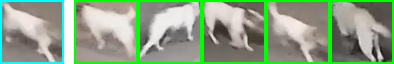
\includegraphics{images/petsearch/ranked_lists/1/collage.jpg}
	\end{subfigure}
	\par\vspace{\abovecaptionskip}
	\begin{subfigure}[b]{\textwidth}
		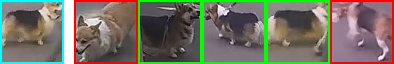
\includegraphics{images/petsearch/ranked_lists/4/collage.jpg}
	\end{subfigure}
	\par\vspace{\abovecaptionskip}
	\begin{subfigure}[b]{\textwidth}
		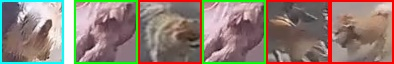
\includegraphics{images/petsearch/ranked_lists/3/collage.jpg}
	\end{subfigure}
	\par\vspace{\abovecaptionskip}
	\begin{subfigure}[b]{\textwidth}
		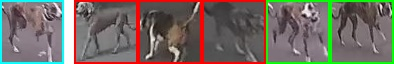
\includegraphics{images/petsearch/ranked_lists/2/collage.jpg}
	\end{subfigure}
	\caption{Пример получаемых ранжированных списков для данных камер видеонаблюдения}
	\label{fig:unicom_ranked}
\end{figure}

Можно видеть, что модель достаточно точно идентифицирует собак по общему внешнему виду, что свидетельствует о применимости подхода метрического обучения для задачи поиска собак.


\section{Анализ результатов}

Таким образом, связь задачи поиска пропавших домашних животных с задачей \reid\ состоит в применимости основных технологий, таких как метрическое обучение, оптимизация ранжирования и использование дополнительной информации.

Однако домен распознавания животных является специфичным, что препятствует прямому переносу общих подходов. Так, для данной сферы не имеется достаточно больших датасетов, имеющих разметку для задачи Re-Id. Таким образом, речь идет не о полном обучении или finetuning-е классических моделей ре-идентификации, а объединении их с дополнительной информацией, специфичной для домена поиска животных.

Так, нейросеть метрического обучения, показывающая высокое качество на некоторых бенчмарках, показывает визуально приемлемые результаты применения в поиске собак. Однако есть и ситуации, свидетельствующие о необходимости использования дополнительной информации для улучшения качества ее работы. Так, например, на \hyperref[fig:confusion]{Рисунке \ref*{fig:confusion}} продемонстрирован случай, когда модель Unicom в качестве ближайшего примера для запроса \ref{fig:confusion_big} выдает изображение \ref{fig:confusion_small}, содержащее собаку, похожую по силуэту, окрасу и типу шерсти, однако относящуюся к другой породе и имеющую другой размер. Для того, чтобы корректно обрабатывать такие ситуации, также может быть полезно внесение в модель априорных знаний о доменной области, позволяющих влиять на решения в спорных ситуациях.

\begin{figure}[ht]
	\centering
	\begin{subfigure}[b]{0.33\textwidth}
		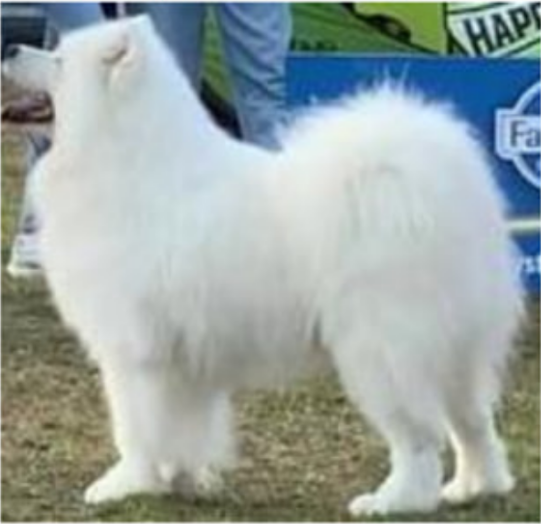
\includegraphics{images/petsearch/confusion/big.png}
		\caption{Самоед}
		\label{fig:confusion_big}
	\end{subfigure}
%	\hfill
	\begin{subfigure}[b]{0.33\textwidth}
		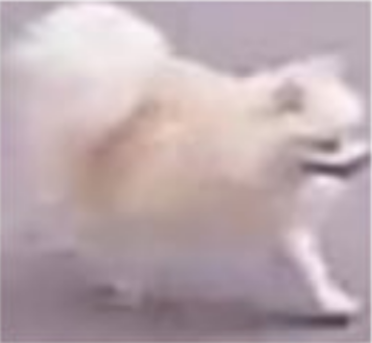
\includegraphics{images/petsearch/confusion/small.png}
		\caption{Чихуахуа}
		\label{fig:confusion_small}
	\end{subfigure}
	\caption{Пример сложного случая}
	\label{fig:confusion}
\end{figure}

Таким образом, проведенные эксперименты свидетельствуют о том, что для оптимальной работы системы поиска на основе Re-Id необходимо учитывать дополнительную информацию, специфичную для доменной области. Это приводит нас к рассмотрению state-of-the-art подхода ре-идентификации CLIP-ReID, позволяющему строить текстовые и визуальные представления.



\endinput
\chapter{Метод CLIP-ReID}
\label{ch:clipreid}

Как упоминалось ранее, для эффективного применения технологий Re-Id в системе поиска, необходимо использовать методы, обрабатывающие на ряду с визуальной информацией некоторую дополнительную. В данном разделе рассмотрим принцип работы state-of-the-art метода решения задачи \reid\ CLIP-ReID \cite{li2023clip}. Он показывает наилучшее качество на одном из бенчмарков задачи ReId $-$ MSMT17 \cite{wei2018person}. Он опирается на мультимодальную модель CLIP \cite{radford2021learning}, позволяющую строить эмбеддинги изображений и текстовых описаний к ним в одном и том же метрическом пространстве. Также здесь применяется техника \textit{prompt tuning}, используемая в методе обучения классификации CoOp \cite{zhou2022learning}, для построения более состоятельных представлений с помощью обучения как визуальной, так и текстовой частей модели CLIP. Схема работы этих методов представлена на \hyperref[fig:clipreid]{Рисунке \ref*{fig:clipreid}}.

\begin{figure}[ht]
	\centering
	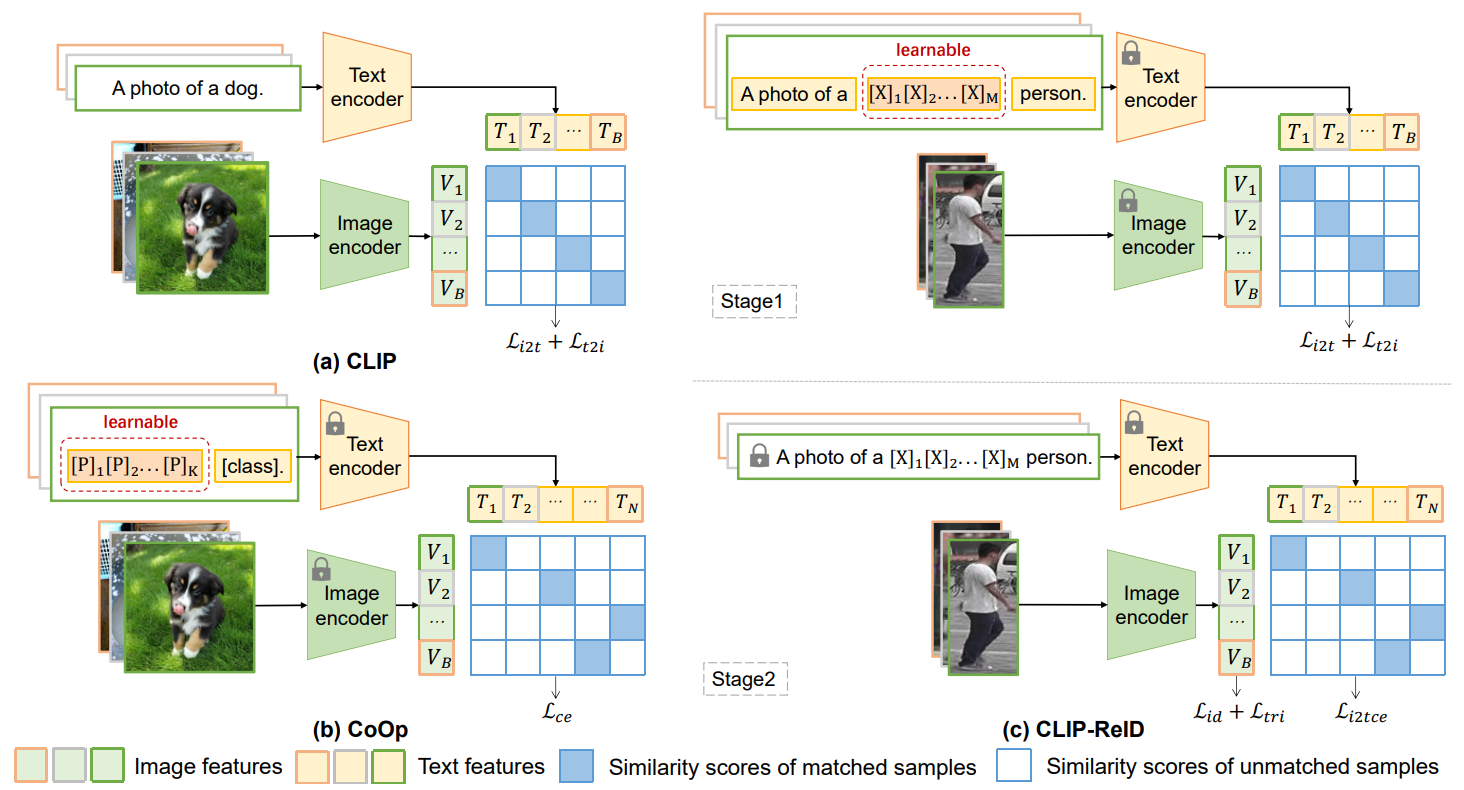
\includegraphics[width=0.9\textwidth]{images/clipreid/scheme.png}
	\caption{Схема работы методов CLIP и CLIP-ReID \cite{radford2021learning}, \cite{li2023clip}}
	\label{fig:clipreid}
\end{figure}


\section{CLIP}

Суть подхода CLIP состоит в построении мультимодальной модели, содержащей энкодер изображений $\mathcal I(\cdot)$ и текстовый энкодер $\mathcal T(\cdot )$. В качестве архитектуры визуального энкодера используется два варианта: ResNet и ViT. В качестве текстового энкодера используется трансформер. Для построения эмбеддинга изображения используется выход визуального энкодера, а для в качестве текстового эмбеддинга выдается представление позиции конца последовательности после преобразования текста трансформером. Затем эти два эмбеддинга проецируются в пространства одинаковой размерности для получения совместных метрических представлений.

Далее на полученные эмбеддинги накладываеются функции потерь, направленные на установление соответствия эмбеддингов текста и картинки, соответствующих одному и тому же объекту. Для объекта батча с индексом $i \in \overline{1, B}$ обозначим текстовое и визуальное представления соответственно $T_i$ и $V_i$. Далее для каждой пары объектов $i$, $j$ считается похожесть, исходя из скалярного произведения:

\begin{equation}
	s (V_i, T_j) = V_i \cdot T_j.
\end{equation}

Лос-функция $\mathcal L_{i2t}$ представляет собой кросс-энтропию, накладываемую в соответствии с классификацией каджого визуального эмбеддинга по похожести с текстовыми эмбеддингами:

\begin{equation}
	\mathcal L_{i2t}(i) = - \log \frac{\exp \left( s(V_i, T_i) \right)}{\sum_{j = 1}^B \exp \left( s(V_i, T_j) \right)}.
\end{equation}

Аналогично определяется функция потерь $\mathcal L_{t2i}$, отвечающая за соответствие текстовых эмбеддингов визуальным:

\begin{equation}
	\mathcal L_{t2i}(i) = - \log \frac{\exp \left( s(V_i, T_i) \right)}{\sum_{j = 1}^B \exp \left( s(V_j, T_i) \right)}.
\end{equation}

Далее они объединяются в итоговую функцию потерь с помощью суммирования:

\begin{eqnarray}
	\mathcal L = \mathcal L_{i2t} + \mathcal L_{t2i}.
\end{eqnarray}

Данный подход позволяет получить модель, способную решать сложные задачи соответствия между текстовыми описаниями и визуальными характеристиками объектов. 

Один из вариантов его развития $-$ метод CoOp, применяющий обучение промптов вместо текстовых описаний при сохранении фиксированными параметров текстового и визуального энкодеров. Данный подход позволяет настравивать CLIP на различные прикладные задачи, связанные с классификацией. Однако для задачи ре-идентификации этот метод не дает прямых преимуществ по сравнению с исходной моделью CLIP, поскольку в отсутствие конкретных текстовых описаний, а также незафиксированном множестве классов, имеется необходимость настройки визуальных эмбеддингов, а не промптов.


\section{CLIP-ReID}

В свою очередь, метод CLIP-ReID адресуется к задаче ре-идентификации. Для этого вводится две стадии настройки предобученной модели CLIP. Авторы показывают, что каждая из этих стадий вносит значимый вклад в прирост качества решения задачи.

\subsection{Первая стадия обучения}

На этом этапе параметры текстового и визуального энкодеров фиксируются. Обучаемыми остается отдельный модуль, называемый \textit{prompt learner} $\mathcal P(\cdot)$. Он формирует входные данные для энкодера $\mathcal T(\cdot)$. Так, для каждого человека, представленного в датасете, формируется описание в формате "A photo of a $[X]_1[X]_2\dots[X]_m$ person". Здесь $[X]_i$ представляет собой обучаемые эмбеддинг токена. Так, при подаче в модель текст разбивается на токены специальным токенизатором, предоставляемым CLIP; для каждого токена строится эмбеддинг. Для токенов $[X]_i$ реальных текстовых токенов нет, именно их представление в виде эмбеддинга является обучаемым параметром модели. 

Каждому человеку соответствует своя обучаемая последовательность эмбеддингов. При этом в батче могут содержаться изображения, соответствующие одному и тому же человеку, поэтому на данном этапе функция потерь модифицируется для учета этого факта:

\begin{equation}\label{eq:Lt2i}
	\mathcal L_{t2i}(y_i) = \frac{-1}{|P(y_i)|} \sum \limits_{p \in P(y_i)} \log \frac{\exp \left( s(V_p, T_{y_i}) \right)}{\sum_{j = 1}^B \exp \left( s(V_j, T_{y_i}) \right)}.
\end{equation}

Итоговая функция потерь также представляет собой сумму текстовой и визуальной кросс-энтропий:

\begin{eqnarray}
	\mathcal L_{stage1} = \mathcal L_{i2t} + \mathcal L_{t2i}.
\end{eqnarray}

Здесь $P(y_i)$ $-$ множество объектов, соответствующих тому же человеку $y_i$. Таким образом с помощью обратного распространения ошибки параметры эмбеддингов промптов оптимизируются для формирования информативных представлений.

\subsection{Вторая стадия обучения}

На втором этапе обучения фиксируются параметры $\mathcal P(\cdot)$ и настраиваются параметры визуального энкодера $\mathcal I(\cdot)$. Здесь совмещаются основные техники решения задачи \reid. Одно из слагаемых представляет собой триплет-лосс:

\begin{equation}\label{eq:Ltri}
	\mathcal L_{tri} = \max \left( d_p - d_n + \rho, 0 \right).
\end{equation}

Второе из слагаемых представляет собой softmax-loss с применением техники сглаживания лейблов, или \textit{label-smoothing},  то есть замены целевого единичного вектора на вектор с малыми, но ненулевыми, значениями на позициях нулей и разности единицы с их суммой на позиции единицы:

\begin{equation}\label{eq:Lid}
	\mathcal L_{id} = \sum \limits_{k = 1}^N q_k \log(p_k),
\end{equation}

где $N$ - количество человек, представленных в датасете, сглаженный индикатор $q_k = (1 - \varepsilon) \delta_{k, y} + \varepsilon N$. Наконец, третье слагаемое отвечает за построение более состоятельных эмбеддингов, соответствующих текстовым промптам. Здесь также используется label smoothing:

\begin{equation}\label{eq:Li2tce}
	\mathcal L_{i2tce}(i) = \sum \limits_{k = 1}^N -q_k \log \frac{\exp \left( s(V_i, T_{y_k}) \right)}{\sum_{y_j = 1}^N \exp \left( s(V_i, T_{y_j}) \right)}.
\end{equation}

Итоговая функция потерь в таком случае:

\begin{equation}
	\mathcal L = \mathcal L_{tri} + \mathcal L_{id} + \mathcal L_{i2tce}(i).
\end{equation}

Таким образом, на первой стадии происходит установка соответствий между информацией, заложенной в предобученную модель CLIP, в виде текстовых промптов. На второй же стадии они применяются в качестве регуляризатора для настройки визуальной модели, позволяя использовать все преимущества мультимодальной модели CLIP.







\chapter{Предложенные модификации}
\label{ch:modifications}

В рамках исследования влияния дополнительной информации на качество работы Re-Id моделей рассматривается классическая постановка задачи $-$ ре-идентификация людей. В данном случае возможно воспользоваться публичными датасетами и бенчмарками для сравнения качества, а также существующей дополнительной разметкой к ним. Рассматривается дополнительная информация двух типов.


\section{Семантические атрибуты}

Во-первых, рассматривается разметка данных по семантическим атрибутам. Работа \cite{lin2019improving} предоставляет разметку Market-1501\_Attribute для датасета Market-1501 \cite{zheng2015scalable} по таким категориям, как: пол, возраст длина волос, тип, длина и цвет верхней и нижней частей одежды, наличие сумок и рюкзаков и др. Описания категорий приведены в \hyperref[tab:market_attributes]{Таблице \ref*{tab:market_attributes}}

\begin{table}[]
	\centering
	\caption{Категории семантических атрибутов в Market-1501\_Attribute}
	\begin{tabular}{|l|l|l|}
		\hline
		\multicolumn{1}{|l|}{Признак} & \multicolumn{1}{l|}{Количество значений} & 
		\multicolumn{1}{l|}{Значения}\\ \hline
		Пол & 2 & мужской, женский \\ \hline
		Длина волос & 2 & короткие, длинные \\ \hline
		Длина рукава & 2 & длинные, короткие \\ \hline
		Длина нижней & 2 & длинная, короткая \\
		части одежды & & \\ \hline
		Тип нижней & 2 & брюки, юбка \\
		части одежды & & \\ \hline
		Наличие головного & 2 & нет, есть \\
		убора & & \\ \hline
		Наличие рюкзака & 2 & нет, есть \\ \hline
		Наличие сумки & 2 & нет, есть \\ \hline
		Наличие дамской & 2 & нет, есть \\
		сумки & & \\ \hline
		Возраст & 4 & подросток, молодой \\
		& & взрослый, старый \\ \hline
		Цвет верхней & 8 & черный, белый \\
		части одежды & & красный, фиолетовый \\
		& & желтый, серый \\
		& & синий, зеленый \\ \hline
		Цвет нижней & 9 & черный, белый \\
		части одежды & & розовый, фиолетовый \\
		& & желтый, серый \\
		& & синий, зеленый \\
		& & коричневый \\ \hline
	\end{tabular}
	\label{tab:market_attributes}
\end{table}

\subsection{Составление промптов на основе атрибутов}

Модель CLIP-ReID опирается на свойство соответствия обучаемых визуальных представлений обучаемым текстовым представлениям. Благодаря двухстадийному обучению удается сохранить заложенную в мультимодальную модель CLIP информацию и использовать ее для регуляризации и улучшения состоятельности эмбеддингов.

В случае же наличия разметки по семантическим атрибутам возможно построение текстовых описаний напрямую. Таким образом, вместо обучаемых промптов возможно составление описаний вида "A photo of a teenager girl with long hair wearing a red T-shirt and gray shorts  carrying a backpack"\ или "A photo of an adult man with short hair wearing a gray T-shirt and black shorts".

Таким образом, первая стадия CLIP-ReID опускается; на второй стадии составляются текстовые эмбеддинги из фиксированных описаний.

\subsection{Label smoothing на основе атрибутов на первой стадии}

В данном варианте рассматривается внесение изменений в функцию потерь первой стадии обучения (\hyperref[eq:Lt2i]{Формула \ref*{eq:Lt2i}}). Для учета информации о похожести людей, имеющих совпадающие значения некоторых атрибутов, предлагается добавление к маске соответствия ID человека маски соответствия атрибутов.

\begin{equation}
	\mathcal L_{t2i}(i) = \frac{1}{|P(y_i)|} \sum \limits_{k = 1}^B -q_k \log \frac{\exp \left( s(V_k, T_i) \right)}{\sum_{j = 1}^B \exp \left( s(V_j, T_i) \right)}.
\end{equation}

Здесь $q_k = (1 - \lambda)\delta_{ik} + \lambda m_{ik}$, где $m_{ik}$ есть доля совпадающих значений атрибутов, $\lambda$ - гиперпараметр.

\subsection{Label smoothing на основе атрибутов на обеих стадиях}

Также возможно расширение этого метода на все этапы обучения. На второй стадии вводятся изменения в правила применения label smoothing. Так, в \hyperref[eq:Lid]{Формуле \ref*{eq:Lid}} и \hyperref[eq:Li2tce]{Формуле \ref*{eq:Li2tce}} коэффициенты кросс-энтропии $q_k$ будут выражаться как $q_k = (1 - \lambda)\delta_{ik} + \lambda m_{ik}$. 

В \hyperref[eq:Ltri]{Формуле \ref*{eq:Ltri}} расстояния до негативных примеров корректируются пропорционально маске сответствия атрибутов:

\begin{equation}
	\mathcal L_{tri} (i) = \max \left( d_p - m_{in} \cdot d_n + \rho, 0 \right).
\end{equation}

Таким образом, при подборе ближайшего негативного примера с помощью hard-batch triplet mining будет увеличиваться приоритет тех объектов, соответствие атрибутов с которыми меньше.


\section{Ключевые точки}

Другой тип рассматриваемой дополнительной информации $-$ разметка изображений людей по ключевым точкам согласно задаче оценки позы, или \textit{pose estimation}. В одном из стандартных вариантов такая разметка содержит 17 ключевых точек, соответствующих лицу, частям тела и суставам.

\subsection{Обучаемый энкодер ключевых точек}

В данном варианте рассматривается использование предразметки ключевых точек для изображений датасета Market-1501, полученное с помощью метода, основанного на HRNet \cite{sun2019deep} $-$ state-of-the-art модели pose estimation. Для обработки данной разметки добавляется отдельный обучаемый энкодер, состоящий из четырех полносвязных слоев. 

Таким образом, на выходе модели имеется три эмбеддинга: текстовый, визуальный и ключевых точек. Последний применяется в качестве регуляризатора для визаульного эмбеддинга. А именно, перед проекцией в общее CLIP-пространство эмбеддинги изображения и ключевых точек конкатенируются. После этого линейный слой отображает их в общее пространство.

\subsection{Регуляризация эмбеддингом модели pose estimation}

Другой вариант использования эмбеддинга ключевых точек $-$ включение эмбеддинга модели pose estimation напрямую перед этап проекции в общее пространство. Таким образом, есть возможность использовать более информативное представление, извлекаемое напрямую из изображения, чем с помощью обучаемого энкодера разметки.

К сожалению, использовать этот эмбеддинг в CLIP-режиме, то есть строя соответствие между тремя, а не двумя, типами эмбеддингов, является более сложной задачей. Действительно, для наделения экнодера ключевых точек таким свойством соответствия нужно более глубоко повторять процесс обучения модели CLIP; в противном случае свойством соответствия в энкодер pose estimation не закладывается. Поэтому в данной работе рассматривается вариант с регуляризацией в виде конкатенации.


\chapter{Результаты экспериментов}
\label{ch:experiments}

Для проведения экспериментов использовались датасет Market-1501, разметка семантических атрибутов Market-1501\_Attribute, а также решение задачи pose estimation с помощью HRNet. В качестве архитектуры визуального энкодера CLIP исползьовалась ResNet-50. Каждый вариант из предложенных модификаций был протестирован с различными значениями гиперпараметров, таких как коэффициент сглаживания в label smoothing, а также количество эпох обучения на второй стадии. Остальные гиперпараметры были зафиксированы на тех же значениях, что и в работа CLIP-ReID. Наилучшими значениями весов лосс-функций также оказались те, что изначально использовались в CLIP-ReID. При этом количество эпох до сходимости модели в некоторых вариантах требовалось большим, чем оригинально. Репозиторий с кодом, использованным для проведения экспериментов, доступен по ссылке: \href{https://github.com/Dentikka/CLIP-ReID}{https://github.com/Dentikka/CLIP-ReID}. 

\section{Сравнение качества методов}

В \hyperref[tab:exp_results]{Таблице \ref*{tab:exp_results}} приведены результаты экспериментов. Полужирным шрифтом обозначен метод с наилучшим качеством - им является исходный метод CLIP-ReID.

Так, в первую очередь было замерено качество базовых методов - CLIP и CLIP-ReID. Также была проверена гипотеза о том, что двухстадийный подход CLIP-ReID может дать дальнейшее улучшение качества при повторении всего процесса обучения еще одну итерацию, благодаря установлению лучшего соответствия между инфорацией разных типов. 

Далее были проведены эксперименты по использованию семантических атрибутов. Так, в одном из экспериментов они использовались для формирования текстовых описаний. В двух других вариантах проверялась возможность применения label smoothing с коэффициентом сглаживания $\lambda = 0.5$, а также модификации метрической лосс-функции умножением на маску соответствия атрибутов. Как видно из таблицы, добавление такого типа сглаживания оказалось излишним и привело к расхождению обучения модели.

Также была проведена серия экспериментов по регуляризации визуального представления на основе информации о позе объекта с помощью конкатенации визуального эмбеддинга с обучаемым эмбеддингом разметки ключевых точек перед проекцией в общее метрическое пространство. 

В одном из вариантов для установления равенства вкладов эбмеддингов изображений и ключевых точек в итоговое представление было добавлено проецирование на единичную сферу, то есть нормировка. В другом варианте, также с целью выравнивания масштаба, производилась номрализация каджого из двух эмбеддингов с помщоью операции, аналогичной батч-нормализации, но не отдельно по каждой компоненте вектора, а нормировакой на одно число $-$ среднюю норму этого вектора. Таким образом построенные эмбеддинги изображения и ключевых точек имели одинаковый порядок масштаба и при этом были распределены более равномерно, а не только на единичной сфере.

Наконец, был рассмотрен вариант с регуляризацией не обучаемым эмбеддингом, а извлекаемым из предобученной модели pose estimation $-$ HRNet, также с применением нормализации. Данная стратегия использовалась только на этапе обучения; на этапе инференса же использовались только визуальные эмбеддинги.

Как следует из \hyperref[tab:exp_results]{Таблицы \ref*{tab:exp_results}}, ни одна из предложенных модификаций не дает улучшения качества по сравнению с исходным методом CLIP-ReID. При этом некоторые методы, основанные на регуляризации, требуют большего числа итераций оптимизации для достижения своего наилучшего результата.

\begin{table}[]
	\centering
	\caption{Сравнение результатов экспериментов}
	\begin{tabular}{|l|l|l|l|l|}
		\hline
		\multicolumn{1}{|l|}{Тип метода} & \multicolumn{1}{l|}{Эксперимент} & \multicolumn{1}{l|}{\#эпох} & 
		\multicolumn{1}{l|}{mAP} & \multicolumn{1}{l|}{CMC@1} \\ \hline
		
		\multirow{3}{*}{\makecell[c]{CLIP-ReID}} & \begin{tabular}[c]{@{}l@{}} Настройка визуальной модели\\ CLIP без первой стадии\end{tabular} & 120 & 88,1 & 94,7 \\ \cline{2-5}
		
		& \begin{tabular}[c]{@{}l@{}} CLIP-ReID с обеими стадиями \end{tabular} & 120 & \textbf{89,8} & \textbf{95,7} \\ \cline{2-5}
		
		& \begin{tabular}[c]{@{}l@{}} Повторение процесса обучения \\ CLIP-ReID 2 раза \end{tabular} & 120 & 89,7 & 95,4 \\ \hline

		\multirow{6}{*}{\makecell[c]{Модификации}} & \begin{tabular}[c]{@{}l@{}} Промпты по атрибутам \\ вместо первой стадии \end{tabular} & 120 & 85,5 & 94,2 \\ \cline{2-5}
		
		& \begin{tabular}[c]{@{}l@{}} Label smoothing по атрибутам \\ на первой стадии \end{tabular} & 120 & 88,9 & 95,6 \\ \cline{2-5}
		
		& \begin{tabular}[c]{@{}l@{}} Label smoothing по атрибутам \\ на обеих стадиях \end{tabular} & 120 & 16,7 & 29,8 \\ \cline{2-5}
		
		& \begin{tabular}[c]{@{}l@{}} Регуляризация эмбеддингом \\ ключевых точек, \\ без нормализации \end{tabular} & 120 & 97,5 & 84,3 \\ \cline{2-5}
		
		& \begin{tabular}[c]{@{}l@{}} Регуляризация эмбеддингом \\ ключевых точек, \\ нормировка \end{tabular} & 360 & 88,1 & 94,9 \\ \cline{2-5}
		
		& \begin{tabular}[c]{@{}l@{}} Регуляризация эмбеддингом \\ ключевых точек, \\ нормализация средней \\ нормой вектора \end{tabular} & 480 & 88,9 & 95,3 \\ \cline{2-5}
		
		& \begin{tabular}[c]{@{}l@{}} Регуляризация эмбеддингом \\ HRNet, нормализация \\ средней нормой вектора \end{tabular} & 480 & 88,1 & 95,1 \\ \hline
	\end{tabular}
	\label{tab:exp_results}
\end{table}


\section{Анализ обученных моделей}

В экспериментах с применением эмбеддинга ключевых точек в качестве регуляризатора для эмбеддинга изображения возможен анализ весов слоя проекции из их пространства в общее пространство, где происходит сопоставление с текстовым эмбеддингом. В частности, при наличии нормализации оба эмбеддинга имеют одинаковый масштаб. Соответственно, возникает возможность сравнить масштаб весов, с которыми они подаются в линейный проектор. 

На \hyperref[fig:proj_weights]{Рисунке \ref*{fig:proj_weights}} приведены гистограммы распределения весов проектора отдельно для компонент эмбеддинга изображения и для ключевых точек. Видно, что в случае обучаемого эмбеддинга (\hyperref[fig:proj_weights_learn]{Рисунок \ref*{fig:proj_weights_learn}}) соответствующие веса концентрируются ближе к нулю по сравнению с компонентами визуального эмбеддинга. При использовании предобученного эмбеддинга HRNet (\hyperref[fig:proj_weights_hrnet]{Рисунок \ref*{fig:proj_weights_hrnet}}) наблюдается та же тенденция, но менее ярко выраженная.

Таким образом, в результате оптимизации модели те ее ветви, которые отвечает за обработку предоставленной дополнительной информации, вносят лишь минимальный вклад в ее работу. Наиболее ярко эта закономерность обнаруживается при построении полностью обучаемого энкодера ключевых точек.

С другой стороны, результаты экспериментов говорят о том, что данная дополнительная ветвь вносит помехи в работу основной модели. В случае, когда данная ветвь является обучаемой, ее вклад минимизируется при оптимизации модели. В случае же работы с фиксированными дополнительными эмбеддингами наблюдается существенный вклад в итоговое представления, однако это сказывается негативным образом на качестве работы модели, которое оказывается хуже, чем в случае с обучаемыми эмбеддингами.

\begin{figure}[ht]
	\centering
	\begin{subfigure}[b]{0.45\textwidth}
		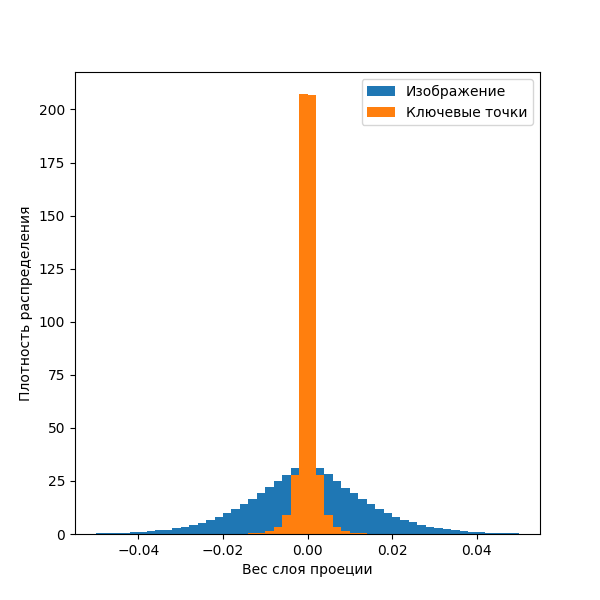
\includegraphics{images/results/analyze_model/concat_normalize.png}
		\caption{Обучаемый эмбеддинг}
		\label{fig:proj_weights_learn}
	\end{subfigure}
	%	\hfill
	\begin{subfigure}[b]{0.45\textwidth}
		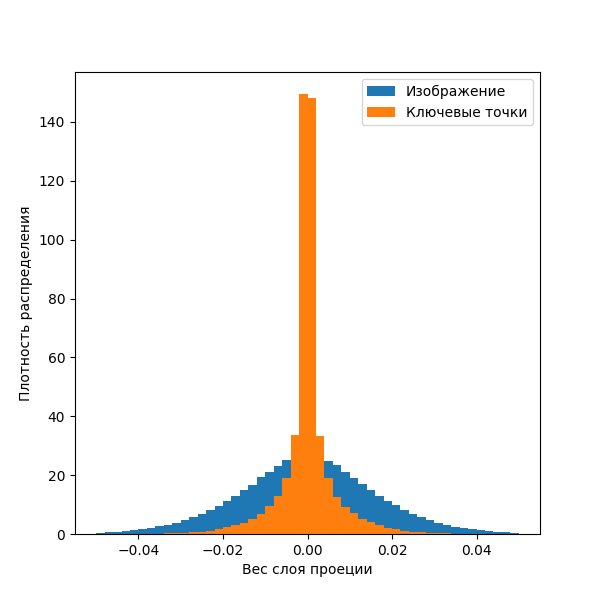
\includegraphics{images/results/analyze_model/concat_hrnet_normalize.png}
		\caption{Эмбеддинг HRNet}
		\label{fig:proj_weights_hrnet}
	\end{subfigure}
	\caption{Распределение весов слоя проекции в общее метрическое пространство. Синим цветом - компоненты эмбеддинга изображения, оранжевым - эмбеддинга ключевых точек.}
	\label{fig:proj_weights}
\end{figure}





\chapter{Заключение}
\label{ch:conclusion}

Таким образом, в работе рассмотрена задача задача \reid, ее научная теория и практические аспекты. Приведена математическая постановка задачи; проведен обширный анализ методов ее решения, а также областей их применимости. Рассмотрено реализованное автором практическое приложение технологий Re-Id. Выявлены пути развития применяемых методов и мотивация к использованию данных путей. Приведен анализ соответствующего базового решения адресованной проблемы, предложены его модификации. Проведены эксперименты по внедрению данных модификаций и анализ их результатов.

Так, ключевую часть решения задачи \reid\ составляют техники метрического обучения. При этом они могут быть дополнены и улучшены с помощью внесения дополнительных знаний о предметной области. Об этом свидетельствуют примеры из практических приложений, а также анализ лидирующих методов.

С другой стороны, улучшение качества с помощью совмещения нескольких техник является сложной задачей. Многие пути ее решения не приводят к успеху. Для построения качественной системы нужна тщательная подготовка данных и построение правильного процесса обучения.

\printbibliography[title=Список использованных источников]

\end{document}